%%%%%%%%%%%%%%%%%%%%%%%%%%%%%%%%%%%%%%%%%
% Beamer Presentation
% LaTeX Template
% Version 1.0 (10/11/12)
%
% This template has been downloaded from:
% http://www.LaTeXTemplates.com
%
% License:
% CC BY-NC-SA 3.0 (http://creativecommons.org/licenses/by-nc-sa/3.0/)
%
%%%%%%%%%%%%%%%%%%%%%%%%%%%%%%%%%%%%%%%%%

%------------------------------------------------------------------------------%
%	PACKAGES AND THEMES
%------------------------------------------------------------------------------%

\documentclass{beamer}

\mode<presentation> {

% The Beamer class comes with a number of default slide themes
% which change the colors and layouts of slides. Below this is a list
% of all the themes, uncomment each in turn to see what they look like.

%\usetheme{default}
%\usetheme{AnnArbor}
%\usetheme{Antibes}
%\usetheme{Bergen}
%\usetheme{Berkeley}
%\usetheme{Berlin}
%\usetheme{Boadilla}
%\usetheme{CambridgeUS}
%\usetheme{Copenhagen}
%\usetheme{Darmstadt}
%\usetheme{Dresden}
%\usetheme{Frankfurt}
%\usetheme{Goettingen}
%\usetheme{Hannover}
%\usetheme{Ilmenau}
%\usetheme{JuanLesPins}
%\usetheme{Luebeck}
\usetheme{Madrid}
%\usetheme{Malmoe}
%\usetheme{Marburg}
%\usetheme{Montpellier}
%\usetheme{PaloAlto}
%\usetheme{Pittsburgh}
%\usetheme{Rochester}
%\usetheme{Singapore}
%\usetheme{Szeged}
%\usetheme{Warsaw}

% As well as themes, the Beamer class has a number of color themes
% for any slide theme. Uncomment each of these in turn to see how it
% changes the colors of your current slide theme.

%\usecolortheme{albatross}
%\usecolortheme{beaver}
%\usecolortheme{beetle}
%\usecolortheme{crane}
%\usecolortheme{dolphin}
%\usecolortheme{dove}
%\usecolortheme{fly}
%\usecolortheme{lily}
%\usecolortheme{orchid}
%\usecolortheme{rose}
%\usecolortheme{seagull}
%\usecolortheme{seahorse}
%\usecolortheme{whale}
%\usecolortheme{wolverine}

% To remove the footer line in all slides, uncomment this line
%\setbeamertemplate{footline}

% To replace the footer line in all slides with a simple slide count,
% uncomment this line
%\setbeamertemplate{footline}[page number]

% To remove the navigation symbols from the bottom of all slides,
% uncomment this line
\setbeamertemplate{navigation symbols}{}
}

% Allows including images
\usepackage{graphicx}

% Allows the use of \toprule, \midrule and \bottomrule in tables
\usepackage{booktabs}

\usepackage{duckuments}

\usepackage{aasmacros}
\usepackage[round,sort,numbers,authoryear]{natbib}
\bibliographystyle{unsrtnat}

\usepackage{wasysym}

\usepackage{cancel}

\usepackage{appendixnumberbeamer}

\newcommand{\thornado}{\texttt{thornado}}
\newcommand{\amrex}{AMReX}

\definecolor{ectblue}{RGB}{40,103,174}
\definecolor{dkgrey}{RGB}{75,75,75}
\setbeamercolor{palette primary}{bg=ectblue,fg=white}
%\setbeamercolor{palette secondary}{bg=dkgrey,fg=white}
%\setbeamercolor{palette tertiary}{bg=dkgrey,fg=white}
\setbeamercolor{palette quaternary}{bg=dkgrey,fg=white}
\setbeamercolor{structure}{fg=dkgrey}
\setbeamercolor{section in toc}{fg=dkgrey}
\setbeamercolor{author in head/foot}{bg=ectblue}
\setbeamercolor{title in head/foot}{bg=dkgrey}
\usepackage[font={color=dkgrey},figurename=Figure,bf]{caption}
\setbeamercolor{normal text}{fg=dkgrey}

\usefonttheme[onlymath]{serif}

% https://tex.stackexchange.com/questions/33969/changing-font-size-of-selected-slides-in-beamer
\newcommand\Fontvi{\fontsize{7}{7.2}\selectfont}
\newcommand\Fontbib{\fontsize{8}{8.2}\selectfont}

%\definecolor{purple}{RGB}{75,50,100}
\definecolor{purple}{HTML}{bf80ff}


\newcommand{\msun}{M_{\odot}}
\newcommand{\red}{\textcolor{red}}
\newcommand{\blue}{\textcolor{blue}}
\newcommand{\magenta}{\textcolor{magenta}}
\newcommand{\p}{\partial}
\newcommand{\pd}[2]{\frac{\p#1}{\p#2}}
\newcommand{\ul}{\underline}
\newcommand{\ol}{\overline}
\newcommand{\bs}{\boldsymbol}
\newcommand{\rsc}{R_{\mathrm{Sc}}}
\newcommand{\nr}{\mathrm{NR}}
\newcommand{\mpns}{M_{\mathrm{PNS}}}
\newcommand{\rpns}{R_{\mathrm{PNS}}}
\newcommand{\rsh}{R_{\mathrm{Sh}}}
\newcommand{\mdot}{\dot{M}}

% --- TITLE PAGE SLIDE ---

\title[MICRA 2023]{A Parametric Study of the SASI Comparing
General Relativistic and Non-Relativistic Treatments}

\author{Samuel J. Dunham}
\date{September 11, 2023}

\begin{document}

\begin{frame}

  \titlepage

\end{frame}

\begin{frame}
%\frametitle{Paper}

  \begin{figure}[htb!]
    \centering
    
\includegraphics[width=\textwidth]{paperTitle.png}
  \end{figure}

  \begin{columns}[c]

    \column{.3\textwidth} % Left column and width
      \centerline{arXiv Link}
      \begin{figure}[htb!]
        \centering
        
\includegraphics[width=0.5\textwidth]{arxivLink.png}
      \end{figure}
    \column{.3\textwidth} % Left column and width
      \centerline{\texttt{thornado}}
      \begin{figure}[htb!]
        \centering
        \includegraphics[width=0.5\textwidth]{thornado.png}
      \end{figure}
    \column{.3\textwidth} % Left column and width
      \centerline{My Website}
      \begin{figure}[htb!]
        \centering
        
\includegraphics[width=0.5\textwidth]{Website.png}
      \end{figure}

  \end{columns}

\end{frame}

% --- TABLE OF CONTENTS SLIDE ---

%\begin{frame}
%\frametitle{Overview}
%
%  \tableofcontents
%
%\end{frame}

% --- PRESENTATION SLIDES ---

\begin{frame}
%\frametitle{Paper}

  \begin{columns}[c]

    \column{.3\textwidth} % Left column and width
      \centerline{$t$}
      \begin{figure}[htb!]
        \centering
        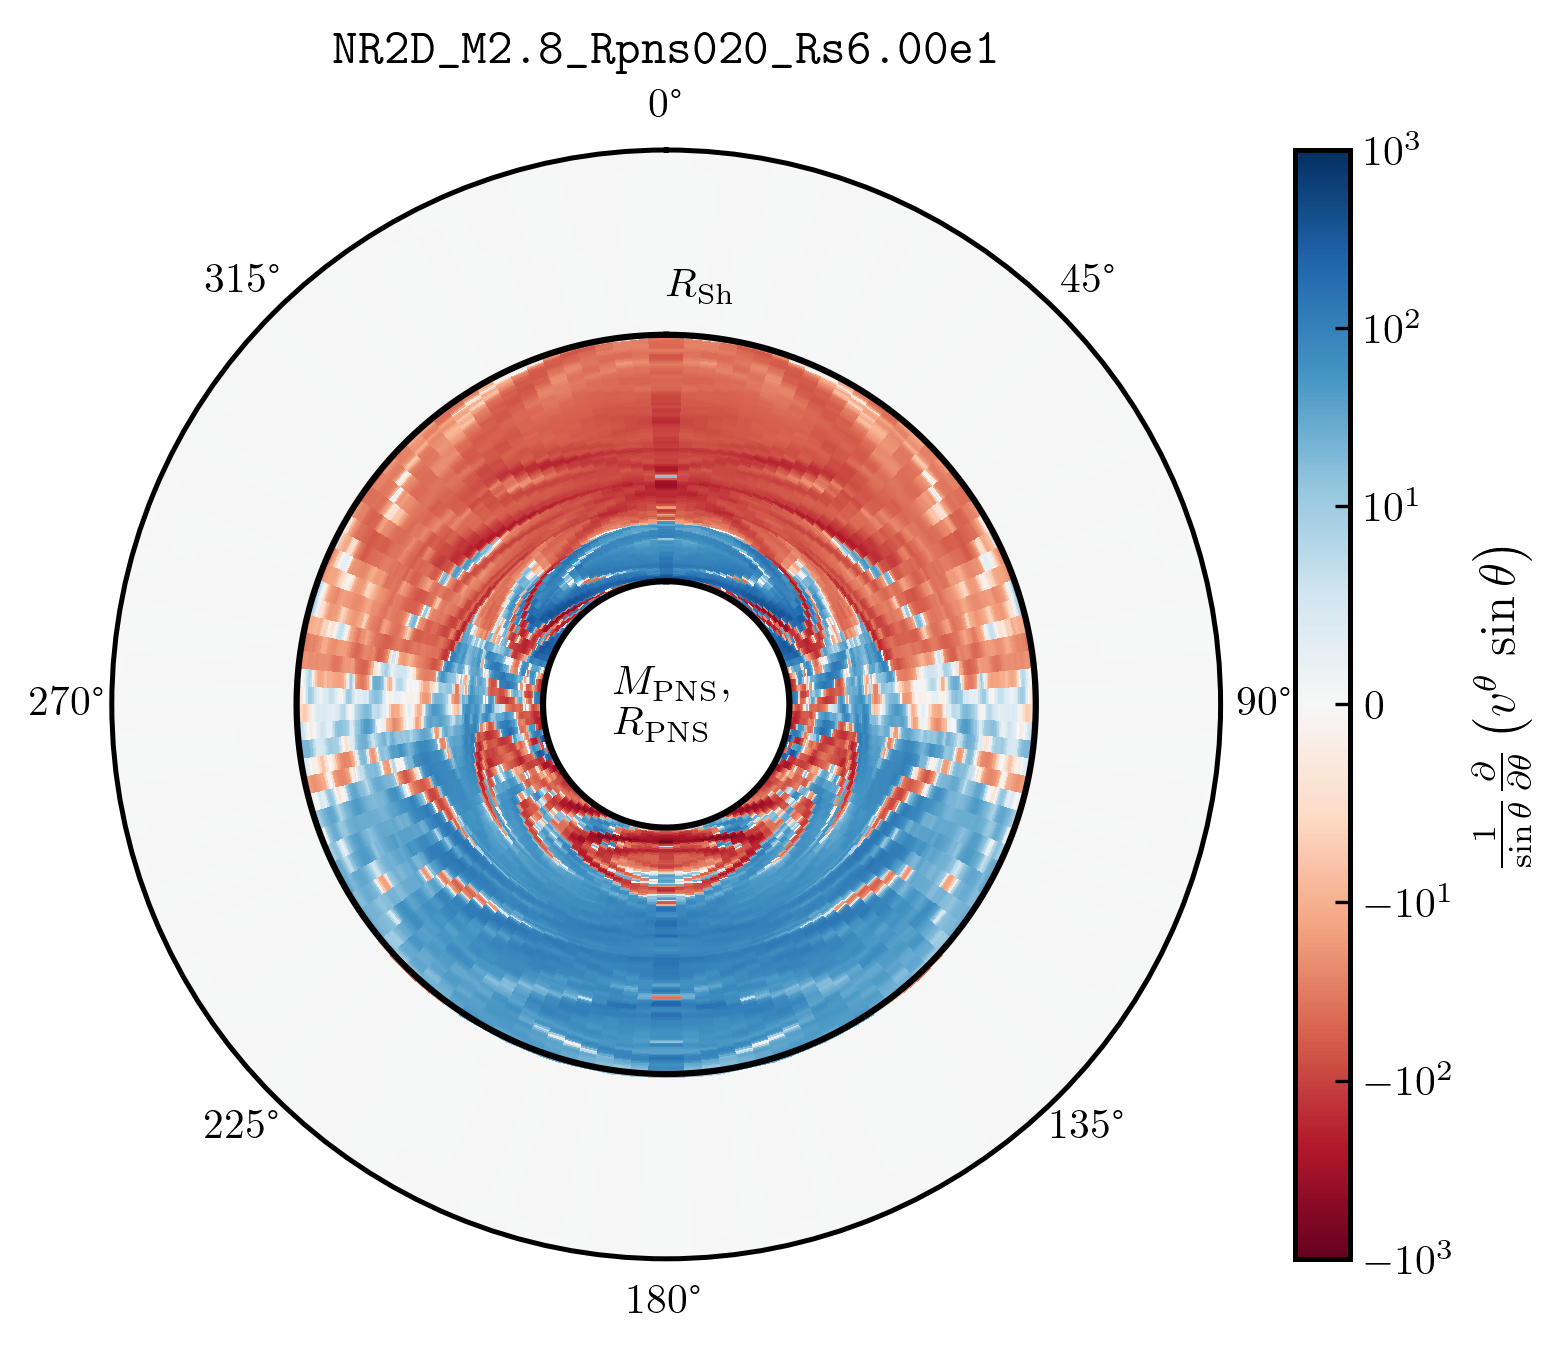
\includegraphics[width=\textwidth]{fig.DivV2_0.00T.png}
      \end{figure}
    \column{.3\textwidth} % Left column and width
      \centerline{$t+0.25\,T$}
      \begin{figure}[htb!]
        \centering
        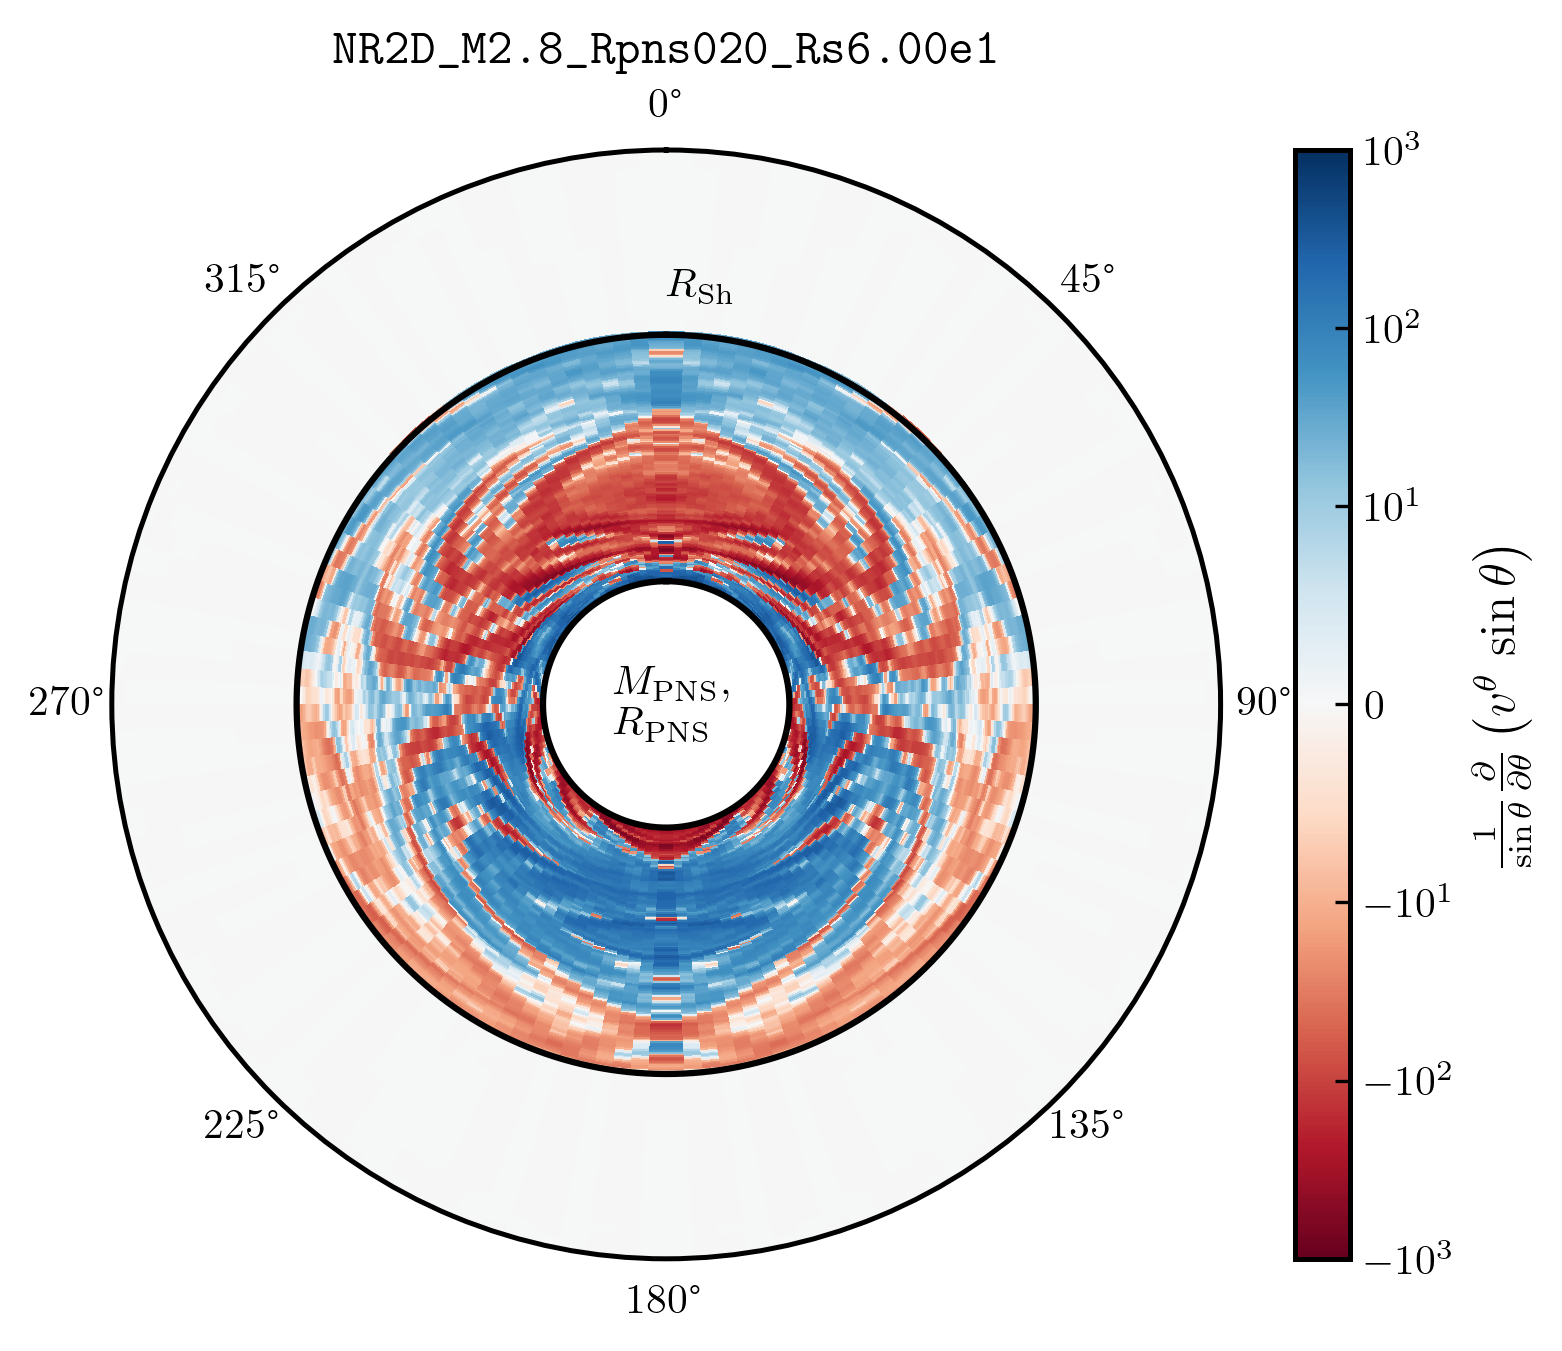
\includegraphics[width=\textwidth]{fig.DivV2_0.25T.png}
      \end{figure}
    \column{.3\textwidth} % Left column and width
      \centerline{$t+0.5\,T$}
      \begin{figure}[htb!]
        \centering
        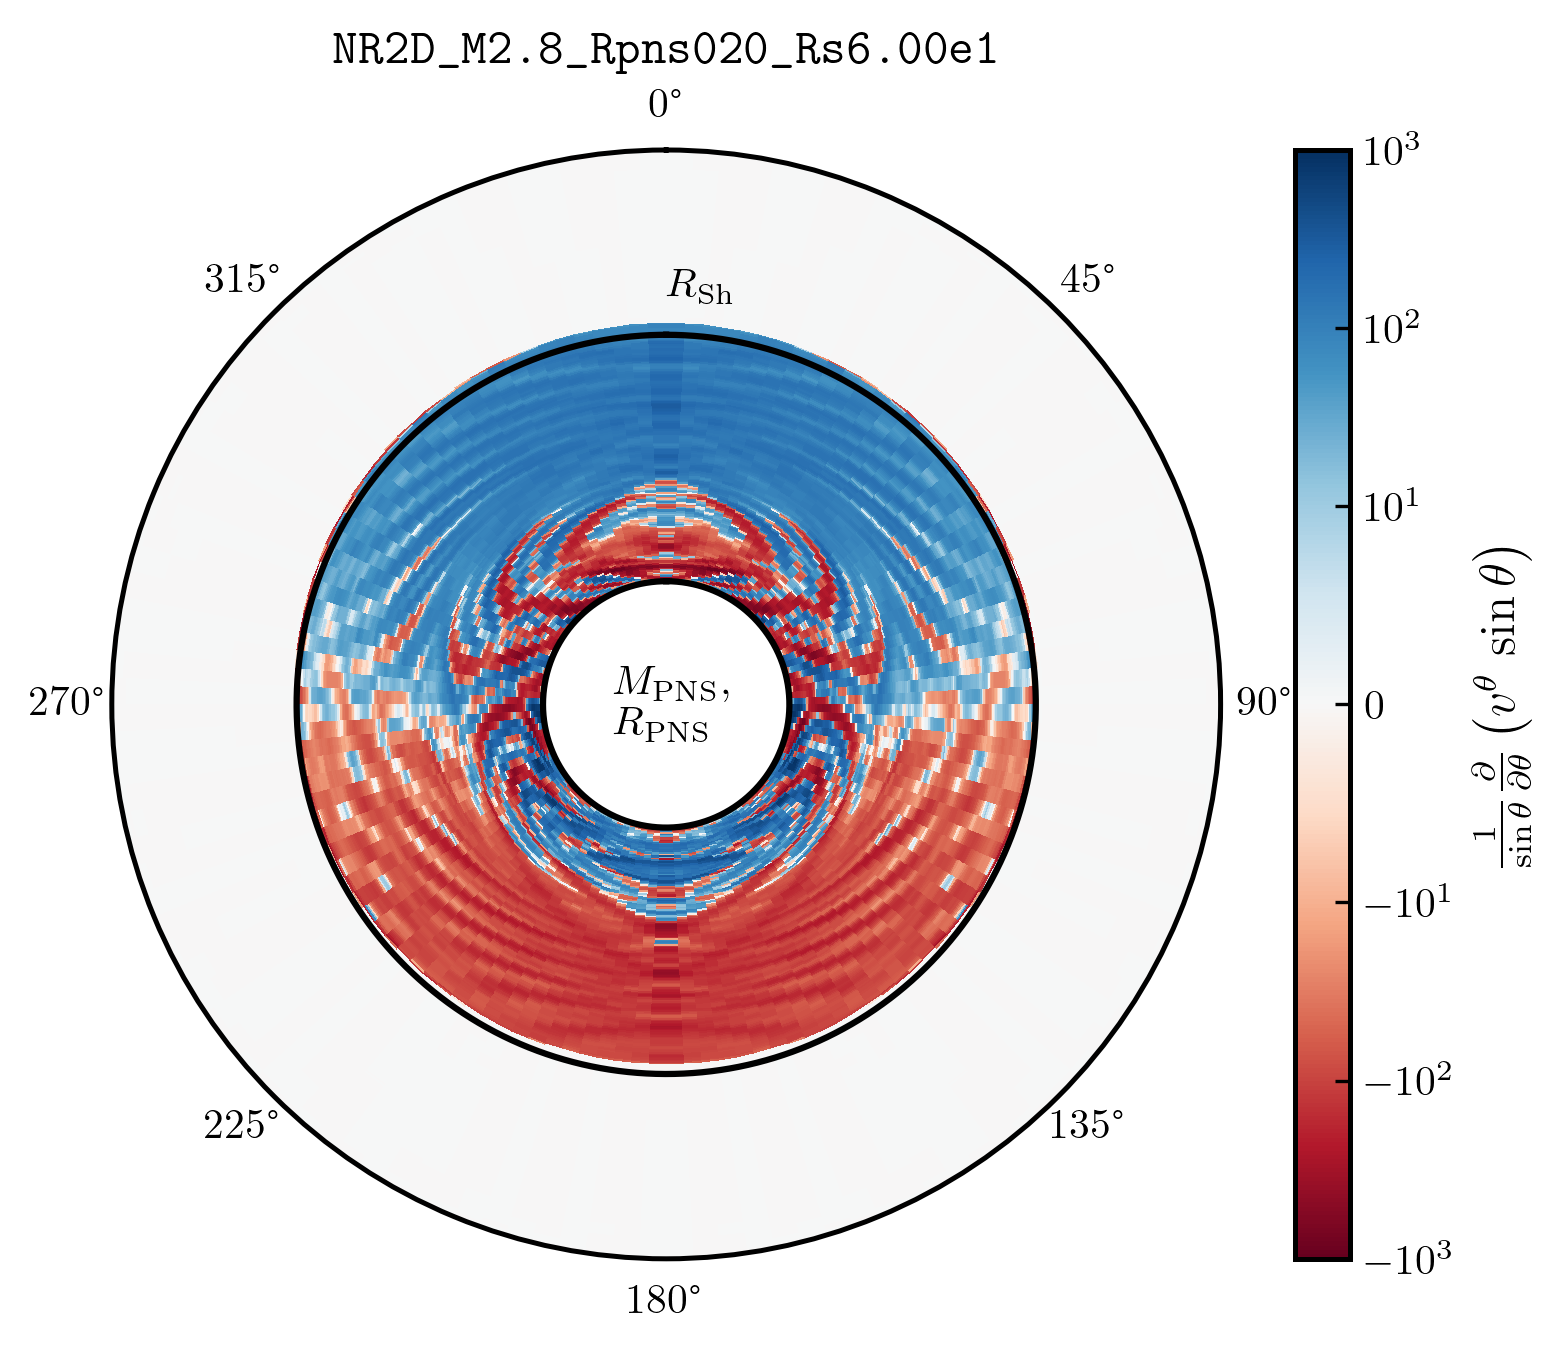
\includegraphics[width=\textwidth]{fig.DivV2_0.50T.png}
      \end{figure}
  \end{columns}

\end{frame}

\begin{frame}

  \begin{figure}[htb!]
    \centering
    \includegraphics[width=0.7\textwidth]%
      {fig.LegendrePowerSpectrum_vst_M2.8_Rpns020_Rsh6.00e1.pdf}
  \end{figure}

\end{frame}

\begin{frame}

  \begin{figure}[htb!]
    \centering
    \includegraphics[width=0.9\textwidth]%
      {fig.SignalSpeedRatios.pdf}
  \end{figure}

\end{frame}

\begin{frame}

  \begin{figure}[htb!]
    \centering
    \begin{minipage}{\textwidth}
      \begin{minipage}{0.3\textwidth}
        \includegraphics[width=\textwidth]%
        {fig.FFT_M1.4_Rpns040_Rsh1.20e2.pdf}
      \end{minipage}
      \hfill
      \begin{minipage}{0.3\textwidth}
        \includegraphics[width=\textwidth]%
        {fig.FFT_M1.4_Rpns040_Rsh1.50e2.pdf}
      \end{minipage}
      \hfill
      \begin{minipage}{0.3\textwidth}
        \includegraphics[width=\textwidth]%
        {fig.FFT_M1.4_Rpns040_Rsh1.75e2.pdf}
      \end{minipage}
      \vfill
      \hspace{2em}
      \begin{minipage}{0.4\textwidth}
        \includegraphics[width=\textwidth]%
        {fig.FFT_M2.8_Rpns020_Rsh6.00e1.pdf}
      \end{minipage}
      \hspace{2em}
      \begin{minipage}{0.4\textwidth}
        \includegraphics[width=\textwidth]%
        {fig.FFT_M2.8_Rpns020_Rsh7.00e1.pdf}
      \end{minipage}
    \end{minipage}
  \end{figure}

\end{frame}

%\begin{frame}
%
%  \begin{figure}[htb!]
%    \centering
%    \begin{minipage}{\textwidth}
%      \begin{minipage}{0.35\textwidth}
%        \includegraphics[width=\textwidth]%
%        {fig.LegendrePowerSpectrum_vst_M1.4_Rpns040_Rsh1.20e2.pdf}
%      \end{minipage}
%      \hfill
%      \begin{minipage}{0.35\textwidth}
%        \includegraphics[width=\textwidth]%
%        {fig.LegendrePowerSpectrum_vst_M2.8_Rpns020_Rsh6.00e1.pdf}
%      \end{minipage}
%      \begin{minipage}{0.4\textwidth}
%        \includegraphics[width=\textwidth]%
%        {fig.FFT_M1.4_Rpns040_Rsh1.20e2.pdf}
%      \end{minipage}
%      \hfill
%      \begin{minipage}{0.4\textwidth}
%        \includegraphics[width=\textwidth]%
%        {fig.FFT_M2.8_Rpns020_Rsh6.00e1.pdf}
%      \end{minipage}
%    \end{minipage}
%  \end{figure}
%
%\end{frame}


\begin{frame}

  \begin{figure}[htb!]
    \centering
    \includegraphics[width=\textwidth]%
      {fig.LegendrePowerSpectrum_MultiPanel_vstOverT.pdf}
  \end{figure}

\end{frame}

\section{Summary, etc.}

\begin{frame}
\frametitle{Conclusions}

  \begin{figure}[htb!]
    \centering
    \includegraphics[width=0.6\textwidth]%
      {fig.LegendrePowerSpectrum_vst_M2.8_Rpns020_Rsh6.00e1.pdf}
  \end{figure}

\end{frame}

\begin{frame}
\frametitle{Conclusions}

  \begin{figure}[htb!]
    \centering
    \includegraphics[width=0.6\textwidth]%
      {fig.GrowthRateComparison.pdf}
  \end{figure}

\end{frame}

\begin{frame}
\frametitle{References}

\Fontbib

  \bibliography{bibfile.bib}

\end{frame}

\begin{frame}
\frametitle{Summary}

  \begin{itemize}
    \item
      Extended study of \citet{bm2006} to include GR
    \item
      Showed that GR leads to longer SASI oscillation period than NR
    \item
      Showed that GR leads to smaller SASI growth rate than NR
    \item
      Found that growth rate is such that $\omega\,T$ is roughly constant
      for some parameter sets: implications for growth rate mechanism
    \item
      Future Work
        \begin{itemize}
          \item
            Extend study to 3D
          \item
            Include GR monopole \citep{mdj2006}
        \end{itemize}
  \end{itemize}

\end{frame}

\appendix

\begin{frame}

  \begin{figure}[htb!]
    \centering
    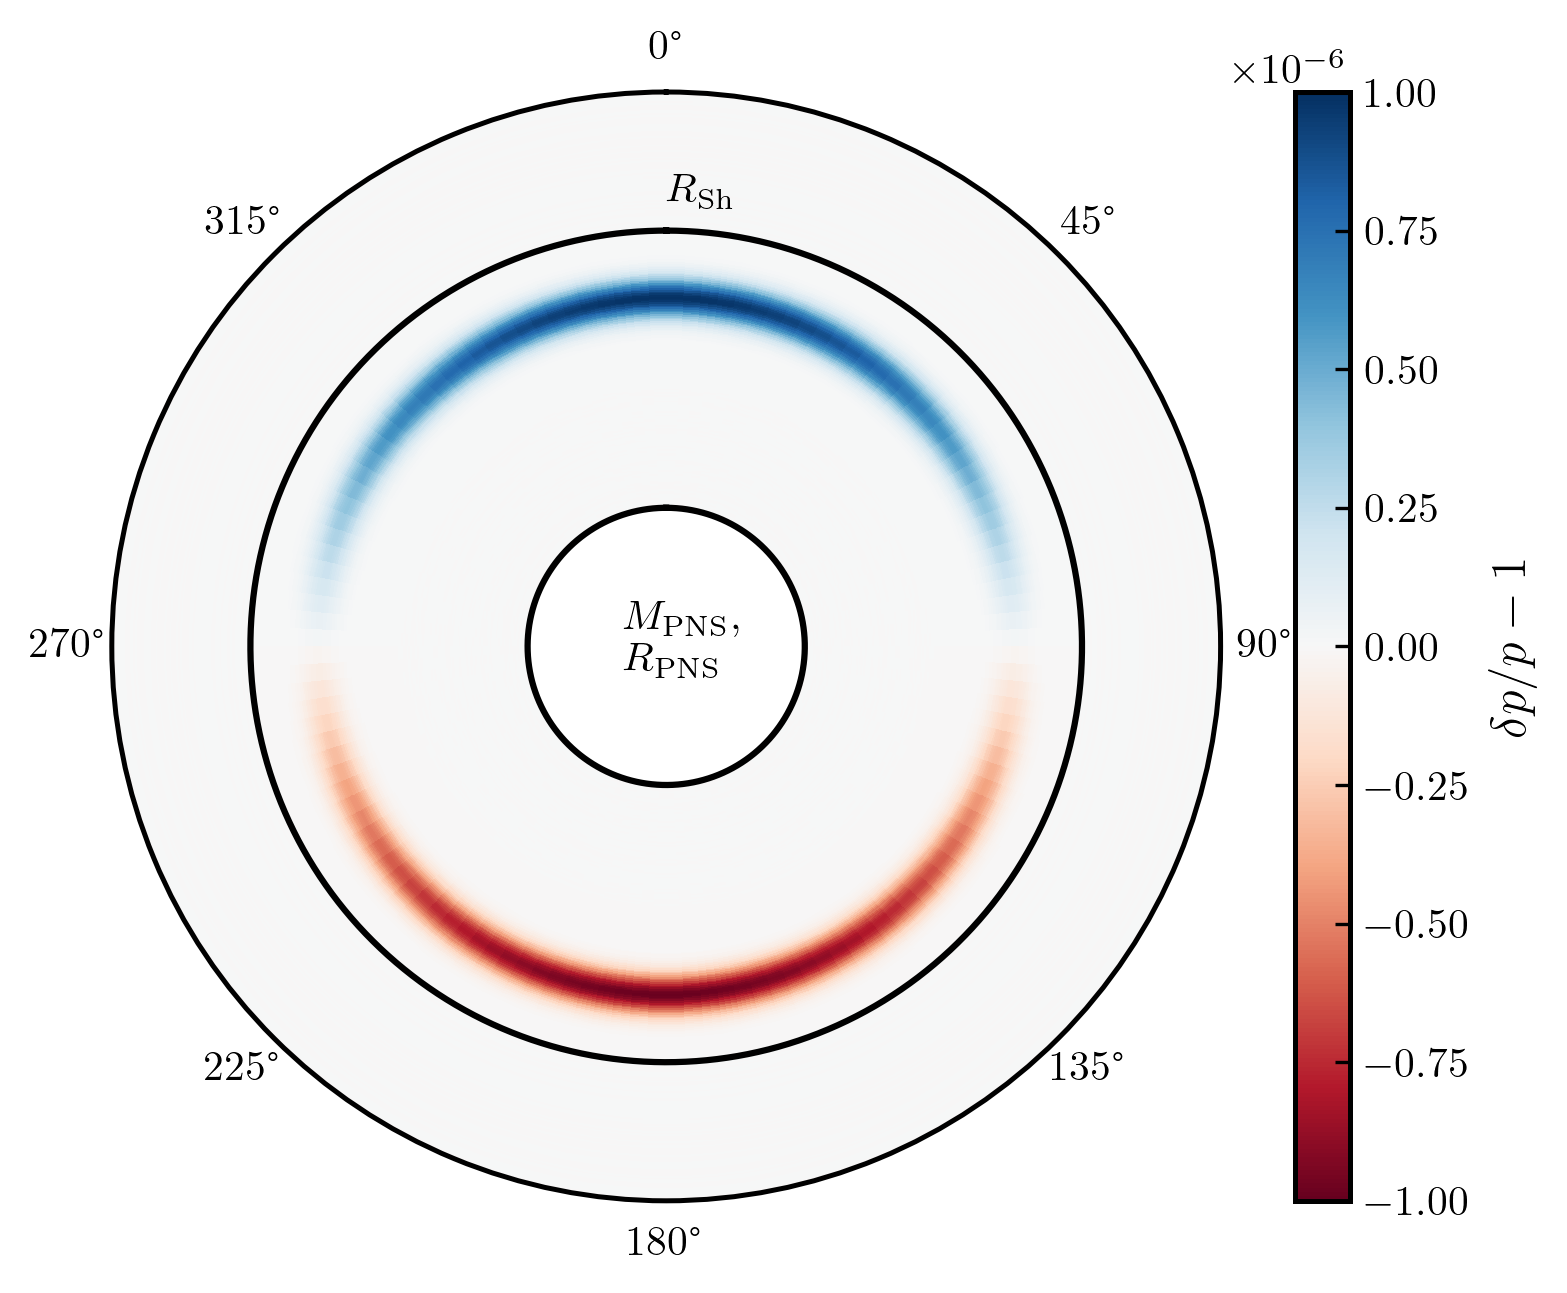
\includegraphics[width=0.8\textwidth]{pert.png}
  \end{figure}

\end{frame}


\begin{frame}

  \begin{figure}[htb!]
    \centering
    \begin{minipage}{\textwidth}
      \begin{minipage}{0.3\textwidth}
        \includegraphics[width=\textwidth]%
        {fig.LegendrePowerSpectrum_vst_M1.4_Rpns040_Rsh1.20e2.pdf}
      \end{minipage}
      \hfill
      \begin{minipage}{0.3\textwidth}
        \includegraphics[width=\textwidth]%
        {fig.LegendrePowerSpectrum_vst_M1.4_Rpns040_Rsh1.50e2.pdf}
      \end{minipage}
      \hfill
      \begin{minipage}{0.3\textwidth}
        \includegraphics[width=\textwidth]%
        {fig.LegendrePowerSpectrum_vst_M1.4_Rpns040_Rsh1.75e2.pdf}
      \end{minipage}
      \vfill
      \hspace{2em}
      \begin{minipage}{0.4\textwidth}
        \includegraphics[width=\textwidth]%
        {fig.LegendrePowerSpectrum_vst_M2.8_Rpns020_Rsh6.00e1.pdf}
      \end{minipage}
      \hspace{2em}
      \begin{minipage}{0.4\textwidth}
        \includegraphics[width=\textwidth]%
        {fig.LegendrePowerSpectrum_vst_M2.8_Rpns020_Rsh7.00e1.pdf}
      \end{minipage}
    \end{minipage}
  \end{figure}

\end{frame}

\begin{frame}

  \begin{enumerate}
    \item[]
      $A:=\frac{1}{\sin\theta}\pd{}{\theta}
        \left(v^{\theta}\,\sin\theta\right)$ \citep{sjf2008}\\[1em]
    \item[]
      $A\left(r,\theta,t\right)
        =\sum\limits_{\ell'=0}^{\infty}G_{\ell'}\left(r,t\right)
        P_{\ell'}\left(\cos\theta\right)$\vspace{0.5em}
    \item[]
      $\hspace{1em}\implies G_{\ell}\left(r,t\right)
        :=\frac{1}{N_{\ell}}\int\limits_{0}^{\pi}
        A\left(r,\theta,t\right)\,P_{\ell}\left(\cos\theta\right)\,
        \sin\theta\,d\theta$\vspace{1em}
    \item[]
      $H_{\ell}\left(t\right)
        :=4\pi\int\limits_{r_{a}}^{r_{b}}
        \left[G_{\ell}\left(r,t\right)\right]^{2}
        \left[\psi\left(r\right)\right]^{6}r^{2}\,dr$
  \end{enumerate}

\end{frame}

\begin{frame}

  \begin{figure}[htb!]
    \centering
    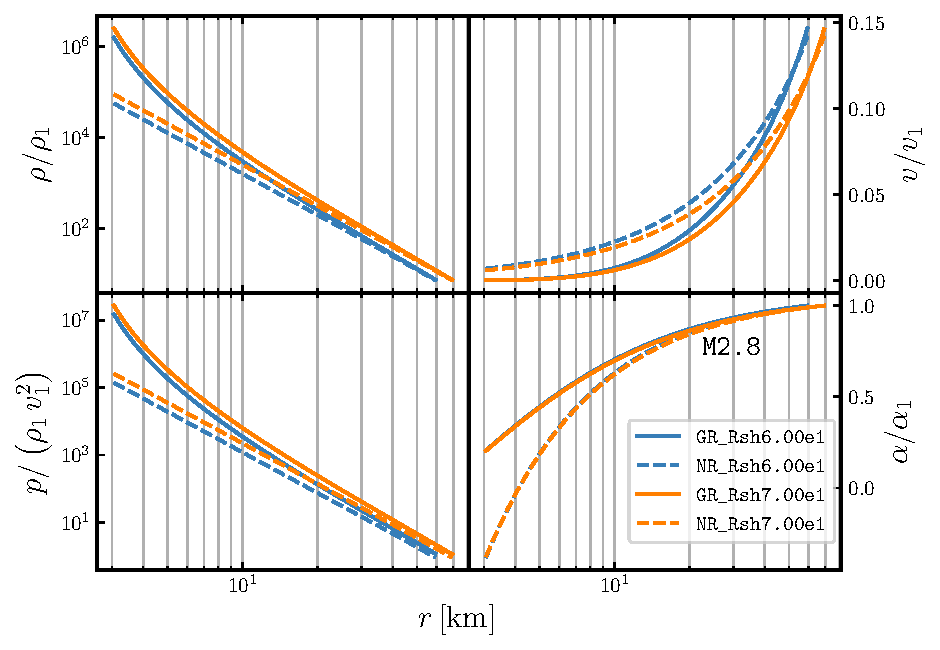
\includegraphics[width=0.8\textwidth]{fig.CompareNRvsGR_SS_M2.8.pdf}
  \end{figure}

\end{frame}

\begin{frame}

  \begin{columns}[c]

    \column{.4\textwidth} % Left column and width

      \begin{itemize}
        \item[]
          Parameters we varied:
          $\xi=\left(\mpns/\msun\right)/\left(\rpns/20\,\mathrm{km}\right)$
          \citep{oo2011},
          $\rsh\left(t=0\right)$
      \end{itemize}

    \column{.55\textwidth} % Right column and width

      \begin{itemize}
        \item[]
            \begin{figure}[ht]
              \centering
              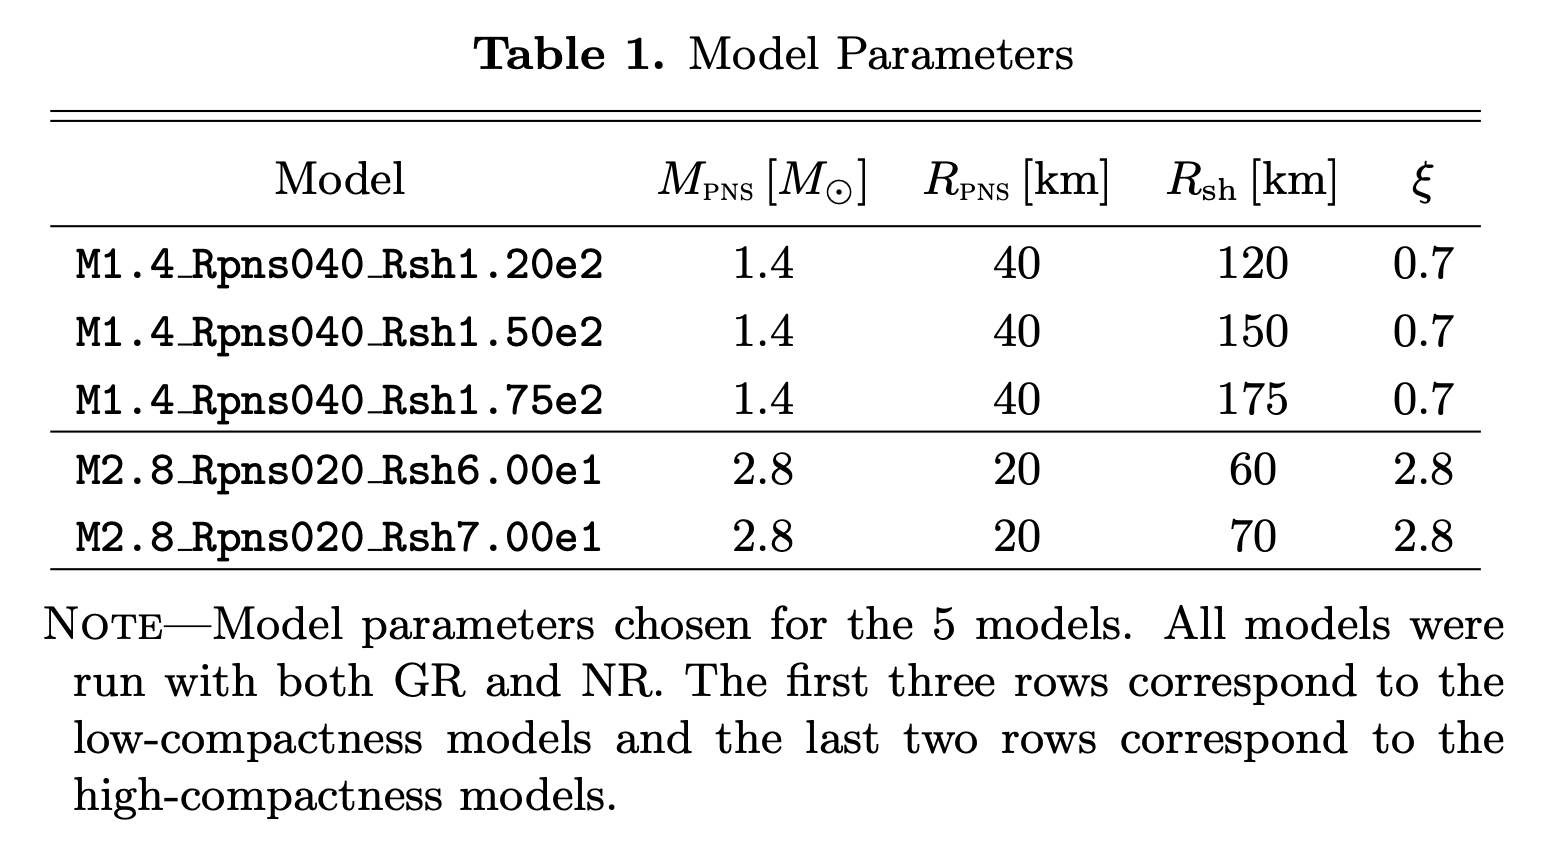
\includegraphics[width=0.9\textwidth]{paramspace.png}
          \end{figure}
      \end{itemize}

  \end{columns}

\end{frame}

\begin{frame}
\frametitle{Conformally-Flat Condition}

  \citet{wmm1996,cc2009}

  \begin{columns}[c]

    \column{.49\textwidth} % Left column and width

    \begin{itemize}[<+->]
      \item[]
        $ds^{2}=-\alpha^{2}\,dt^{2}+\gamma_{ij}\,dx^{i}\,dx^{j}$\\[1em]
      \item[]
        $\gamma_{ij}=\psi^{4}\,\bar{\gamma}_{ij}$\\[1em]
        $1\leq\psi<2$: Conformal factor\\[1em]
        $\bar{\gamma}_{ij}
        =\mathrm{diag}\left(1,r^{2},r^{2}\sin^{2}\theta\right)$\\[1em]
      \item[]
        (Also, maximum slicing condition:
        $K:=\mathrm{Tr}_{\gamma_{ij}}\left(\ul{\ul{K}}\right)=\p_{t}\,K=0$)
    \end{itemize}

    \column{.5\textwidth} % Right column and width

      \begin{figure}[htb!]
        \centering
        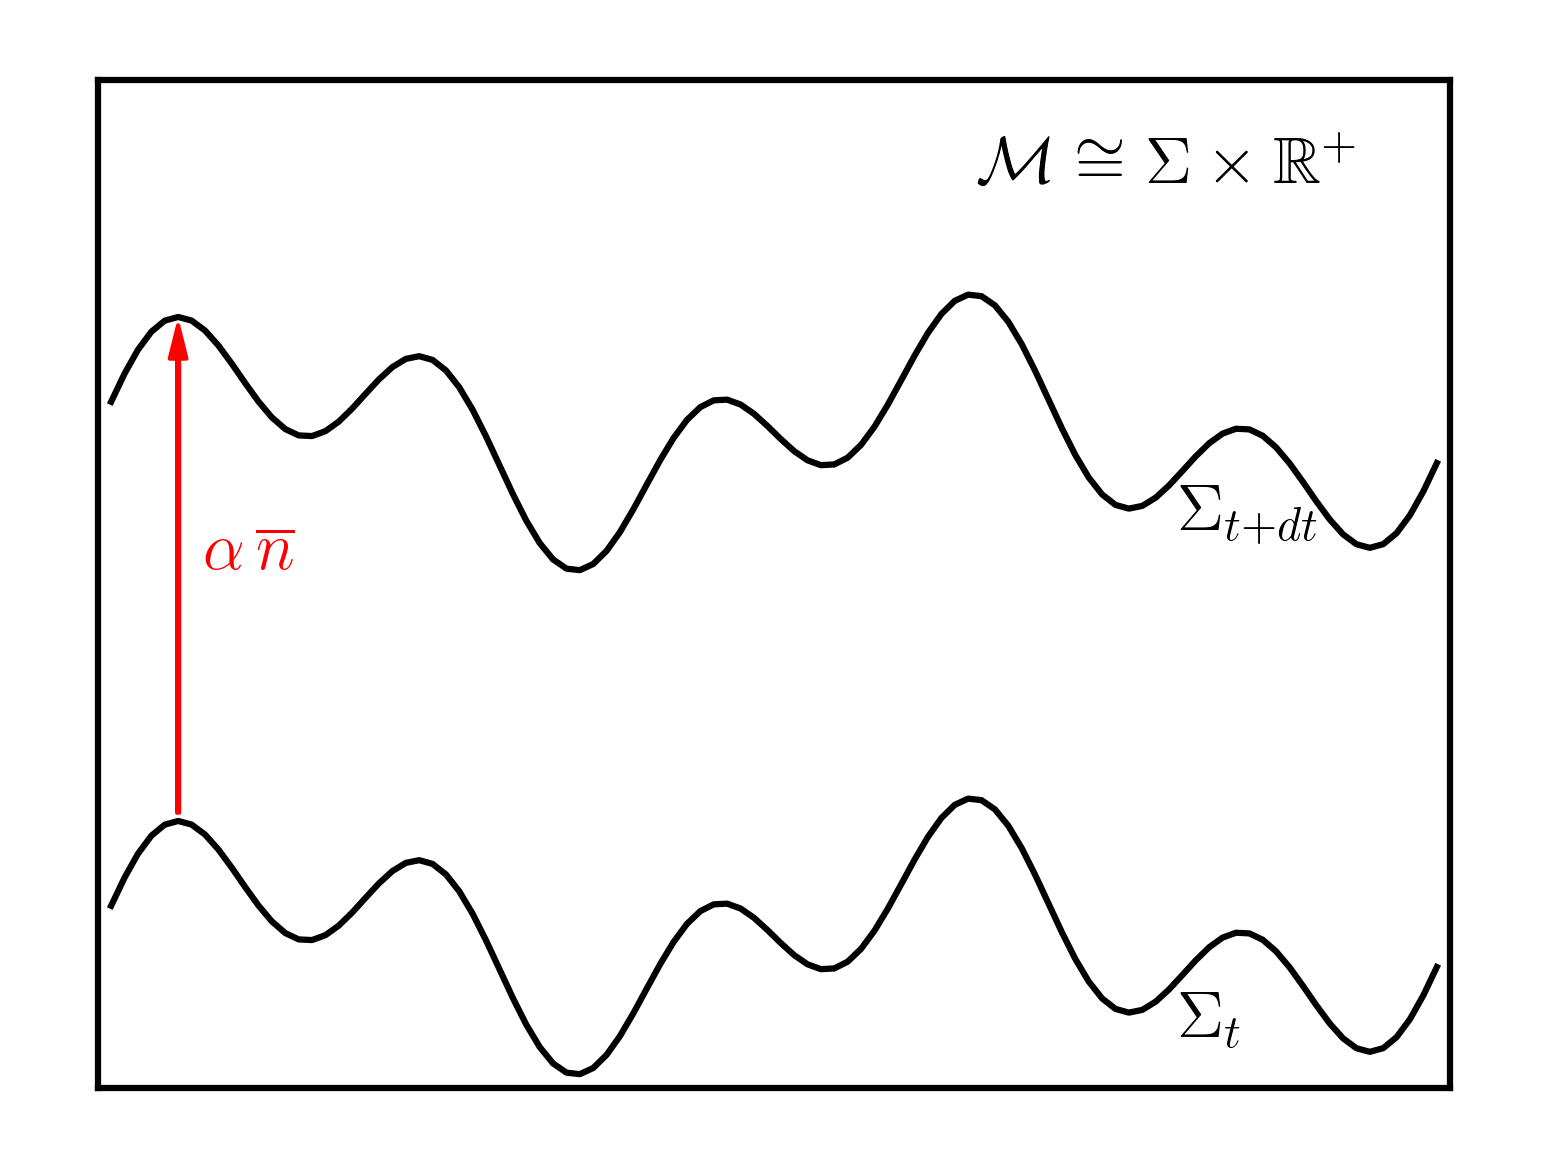
\includegraphics[width=\textwidth]{1+1a.png}
      \end{figure}

  \end{columns}

\end{frame}

\begin{frame}
\frametitle{Isotropic Coordinates ($c=G=1$)}

  \citet{bs2010}\vspace{1em}

  \begin{itemize}[<+->]
    \item[]
      $\alpha\left(r\right)=
      \left(1-\frac{\rsc}{r}\right)\left(1+\frac{\rsc}{r}\right)^{-1}$\\[1em]
    \item[]
      $\psi\left(r\right)=
      1+\frac{\rsc}{r}$\\[1em]
    \item[]
      $r>\rsc:=M/2$\\[1em]
    \item[]
      $\beta^{i}=0$\\[1em]
      $K_{ij}=0$
  \end{itemize}

\end{frame}

\begin{frame}

  \begin{figure}[htb!]
    \centering
    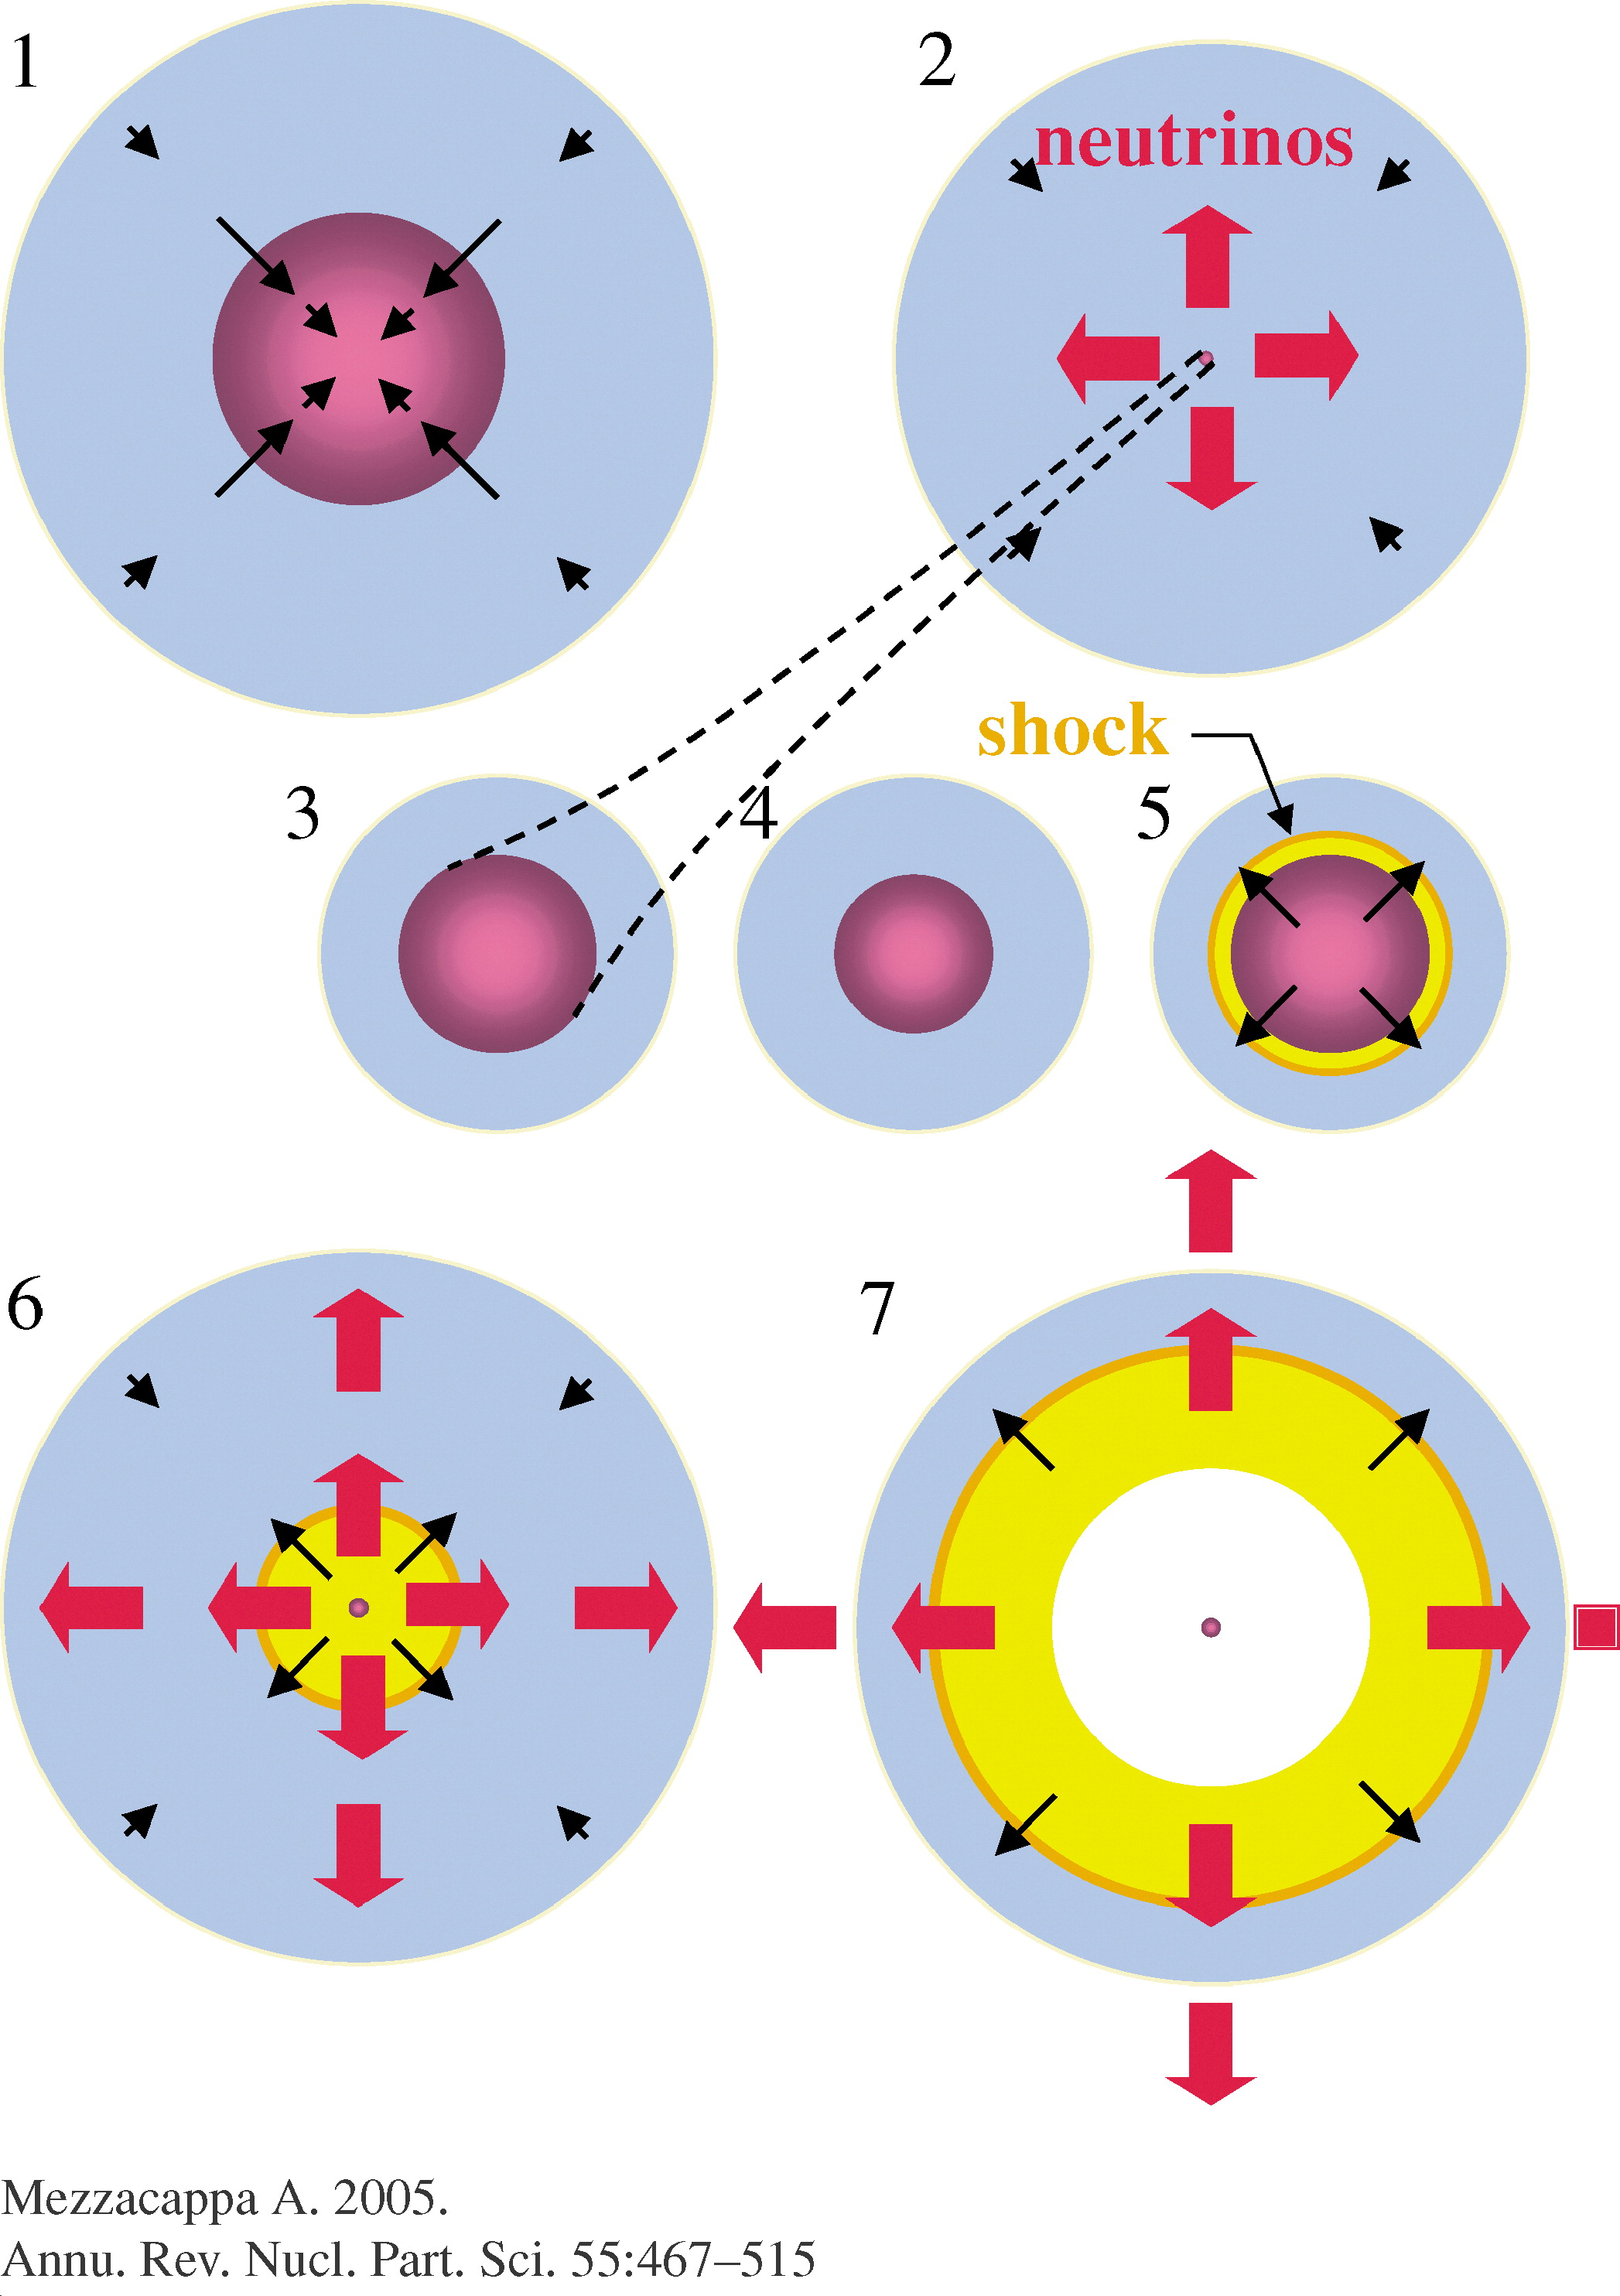
\includegraphics[width=0.45\textwidth]{explosion.jpeg}
  \end{figure}

\end{frame}

\begin{frame}

  \begin{figure}[htb!]
    \centering
    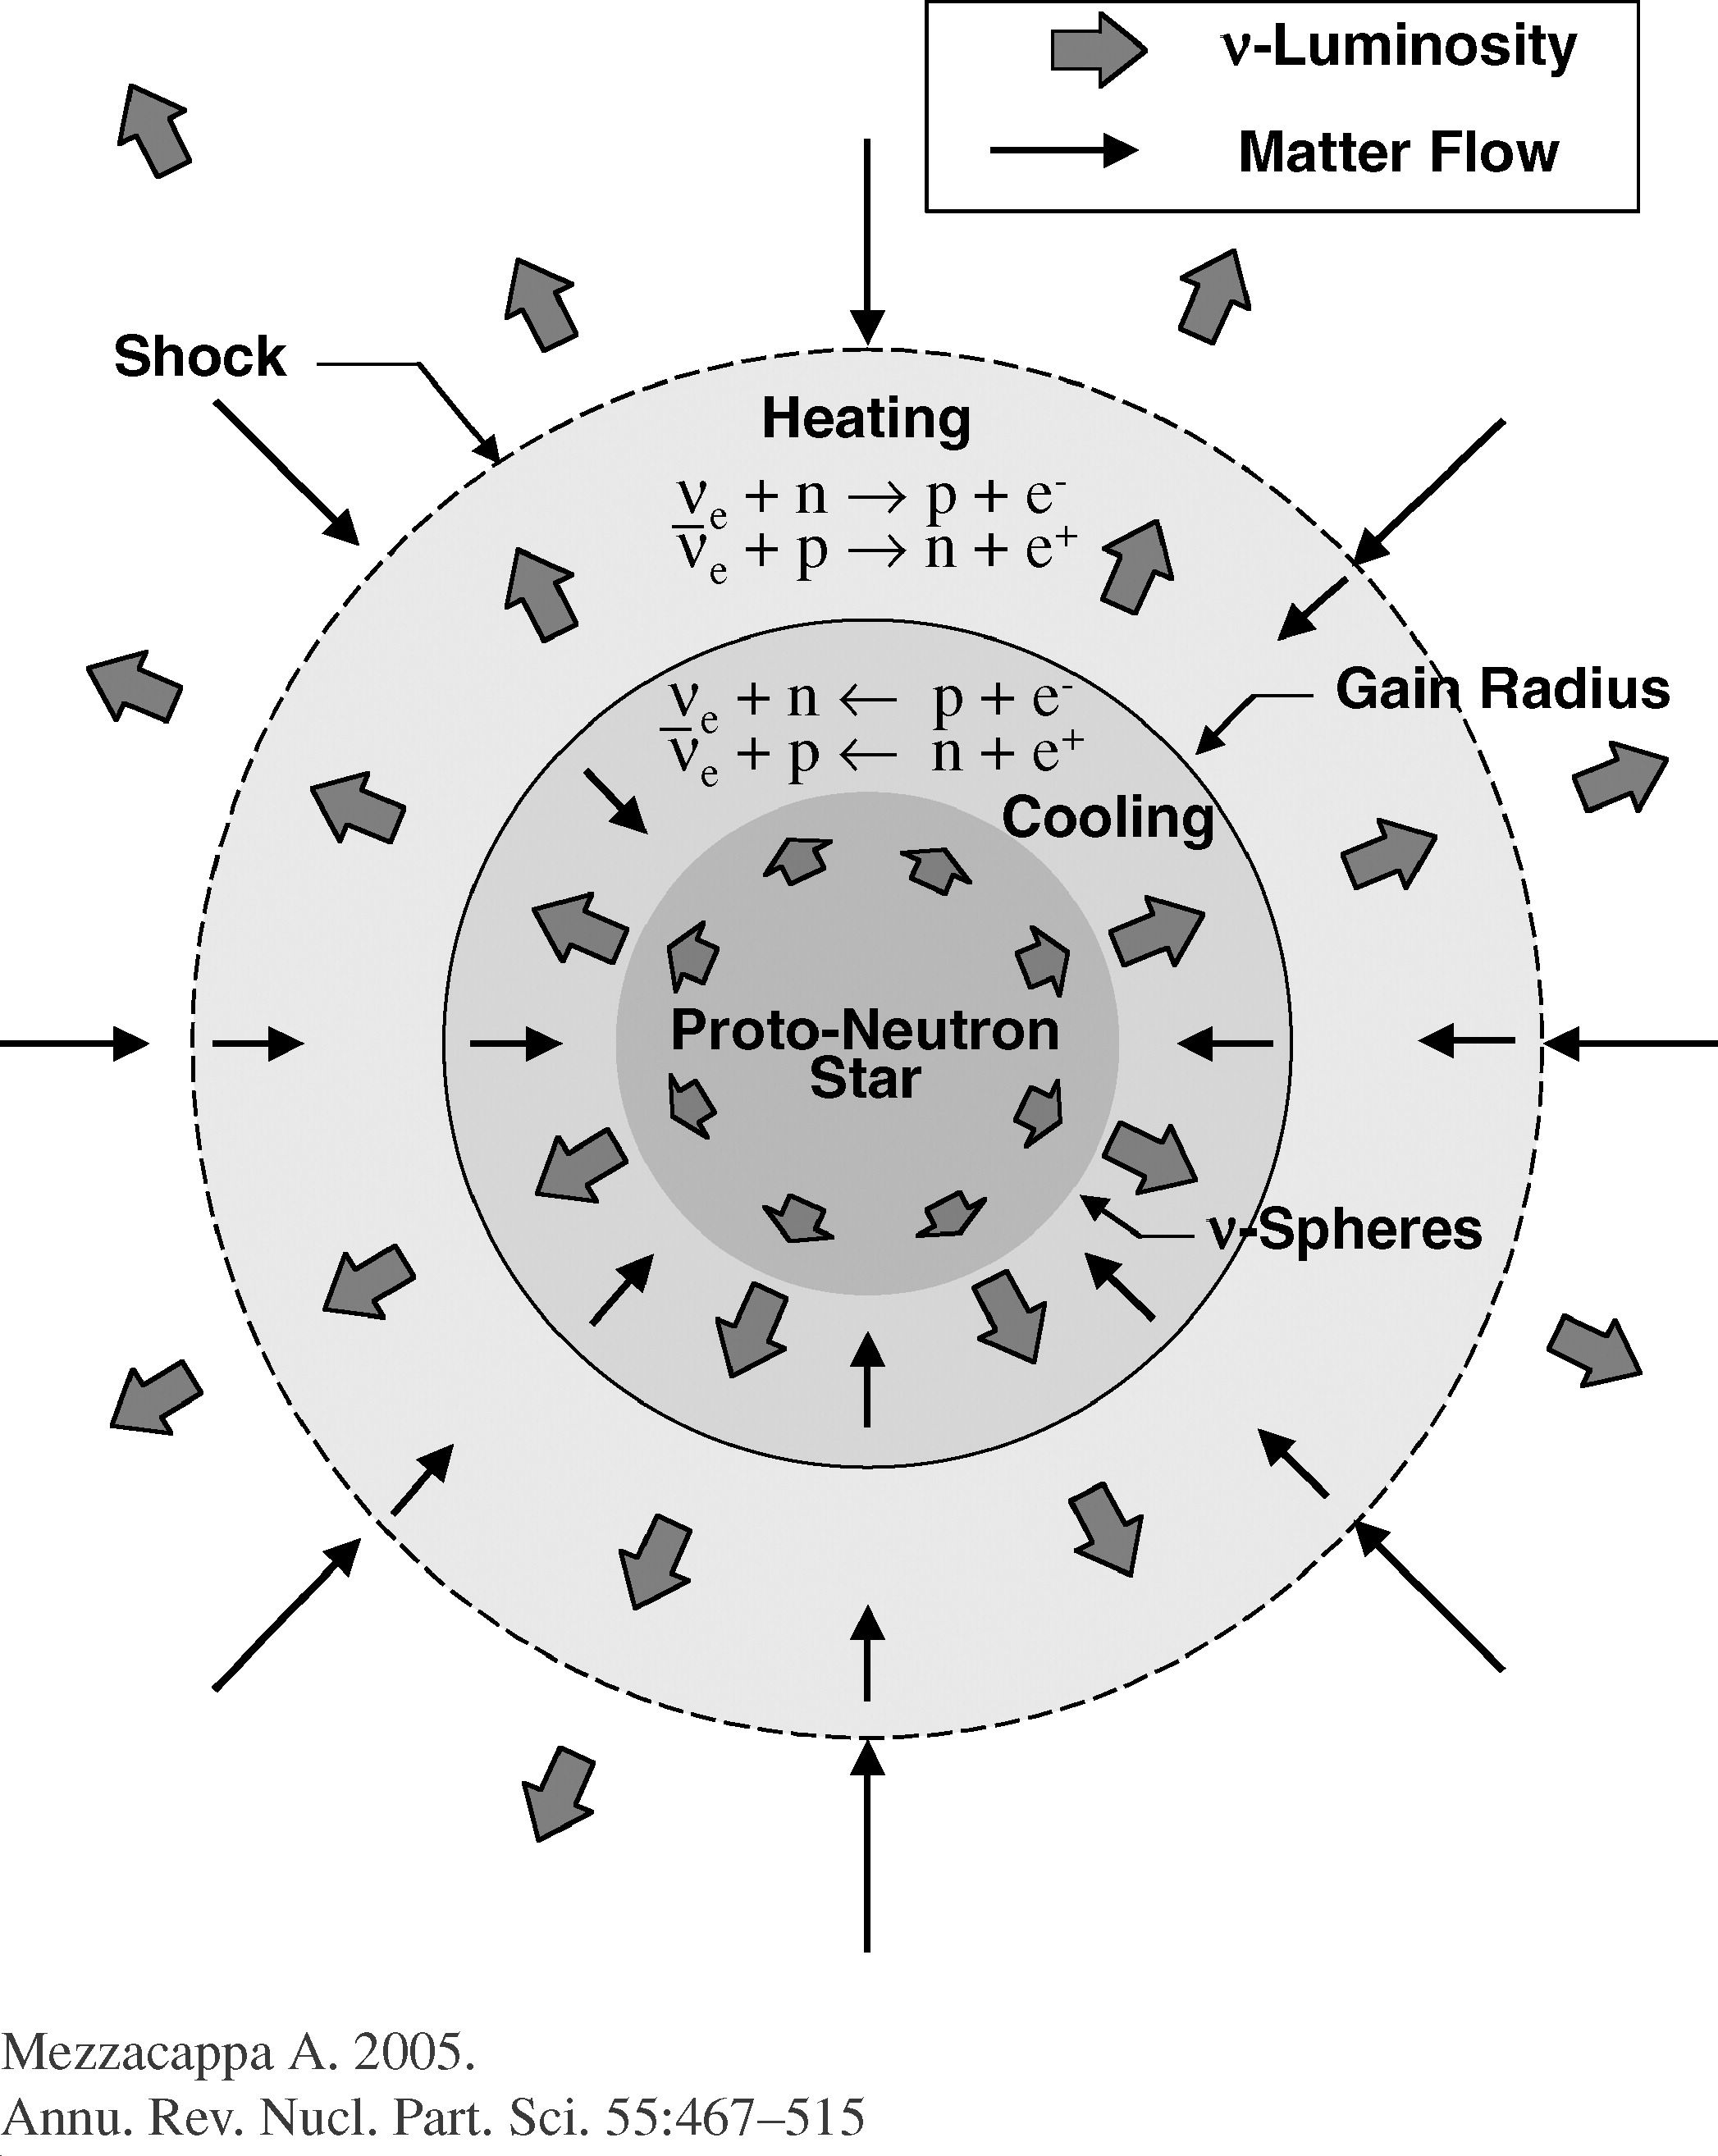
\includegraphics[width=0.5\textwidth]{pns.jpeg}
  \end{figure}

\end{frame}

\begin{frame}

  \begin{figure}[htb!]
    \centering
    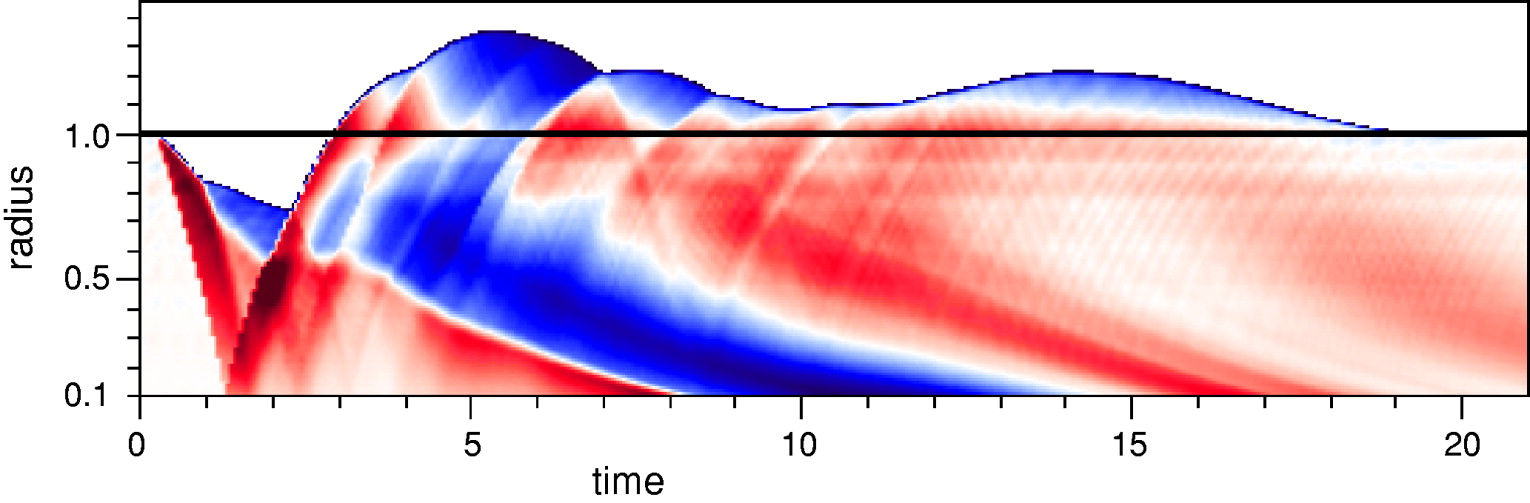
\includegraphics[width=\textwidth]{pressure.jpg}
    \caption{Equilibrium (white), under- (blue), and over- (red) pressure
             \citep{bmd2003}.}
  \end{figure}

\end{frame}

\begin{frame}

  \begin{figure}[htb!]
    \centering
    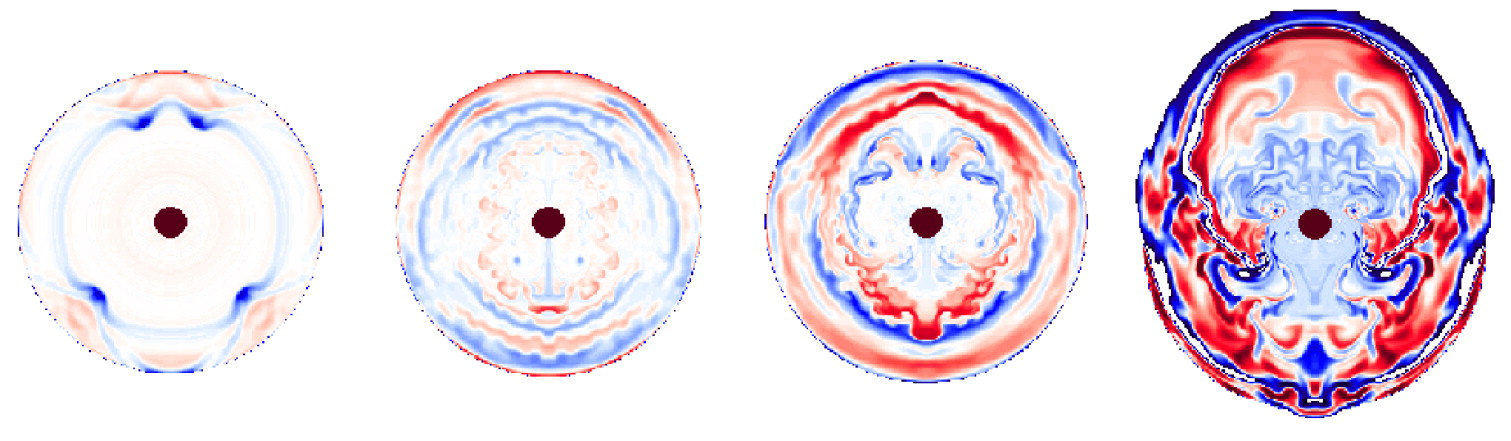
\includegraphics[width=\textwidth]{sasi.jpg}
    \caption{Equilibrium (white), under- (blue), and over- (red) entropy
             \citep{bmd2003}.}
  \end{figure}

\end{frame}

\begin{frame}
\frametitle{$d$+1 Decomposition}

  \begin{columns}[c]

    \column{.49\textwidth} % Left column and width

      \begin{itemize}[<+->]
        \item[]
          $ds^{2}=g_{\mu\nu}\,dx^{\mu}\,dx^{\nu}$\\[1em]
        \item[]
          $\ul{\ul{g}}$: spacetime metric on $\mathcal{M}$\\[1em]
        \item[]
          $g_{\mu\nu}
            =\begin{pmatrix}
             -\alpha^{2}+\beta^{k}\beta_{k} & \beta_{j} \\[1em]
             \beta_{i}   & \gamma_{ij}
             \end{pmatrix}$\\[1em]
        \item[]
          $\ul{\ul{\gamma}}$: spatial three-metric on $\Sigma_{t}$\\[1em]
        \item[]
          $0<\alpha\leq1$: Lapse Function\\[1em]
        \item[]
          $\ol{n}$: Eulerian four-velocity\\[1em]
          ($\ul{\ul{g}}\left(\ol{n},\ol{n}\right)=\ol{n}\cdot\ol{n}=-1$)\\[1em]
        \item[]
          (Also, $\ul{\ul{K}}$: Extrinsic curvature)
      \end{itemize}

    \column{.5\textwidth} % Right column and width

      \begin{figure}[htb!]
        \centering
        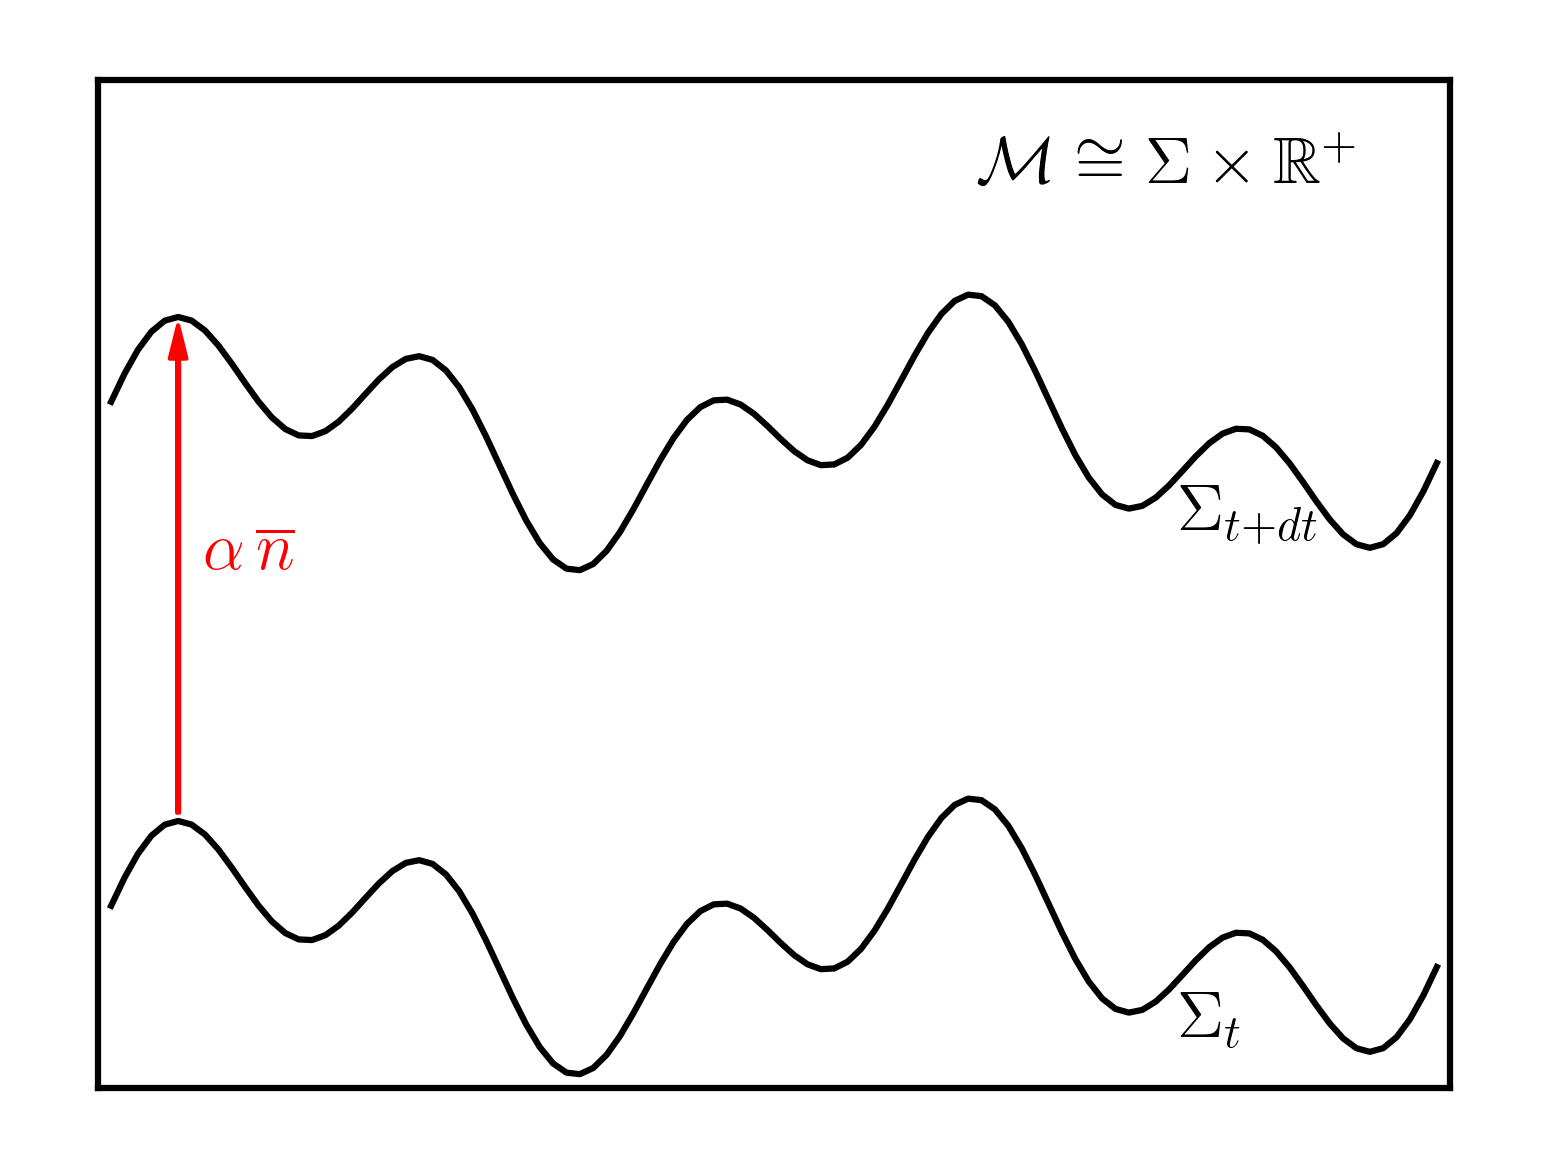
\includegraphics[width=\textwidth]{1+1a.png}
      \end{figure}

  \end{columns}

\end{frame}

\begin{frame}

  \begin{figure}[htb!]
    \centering
    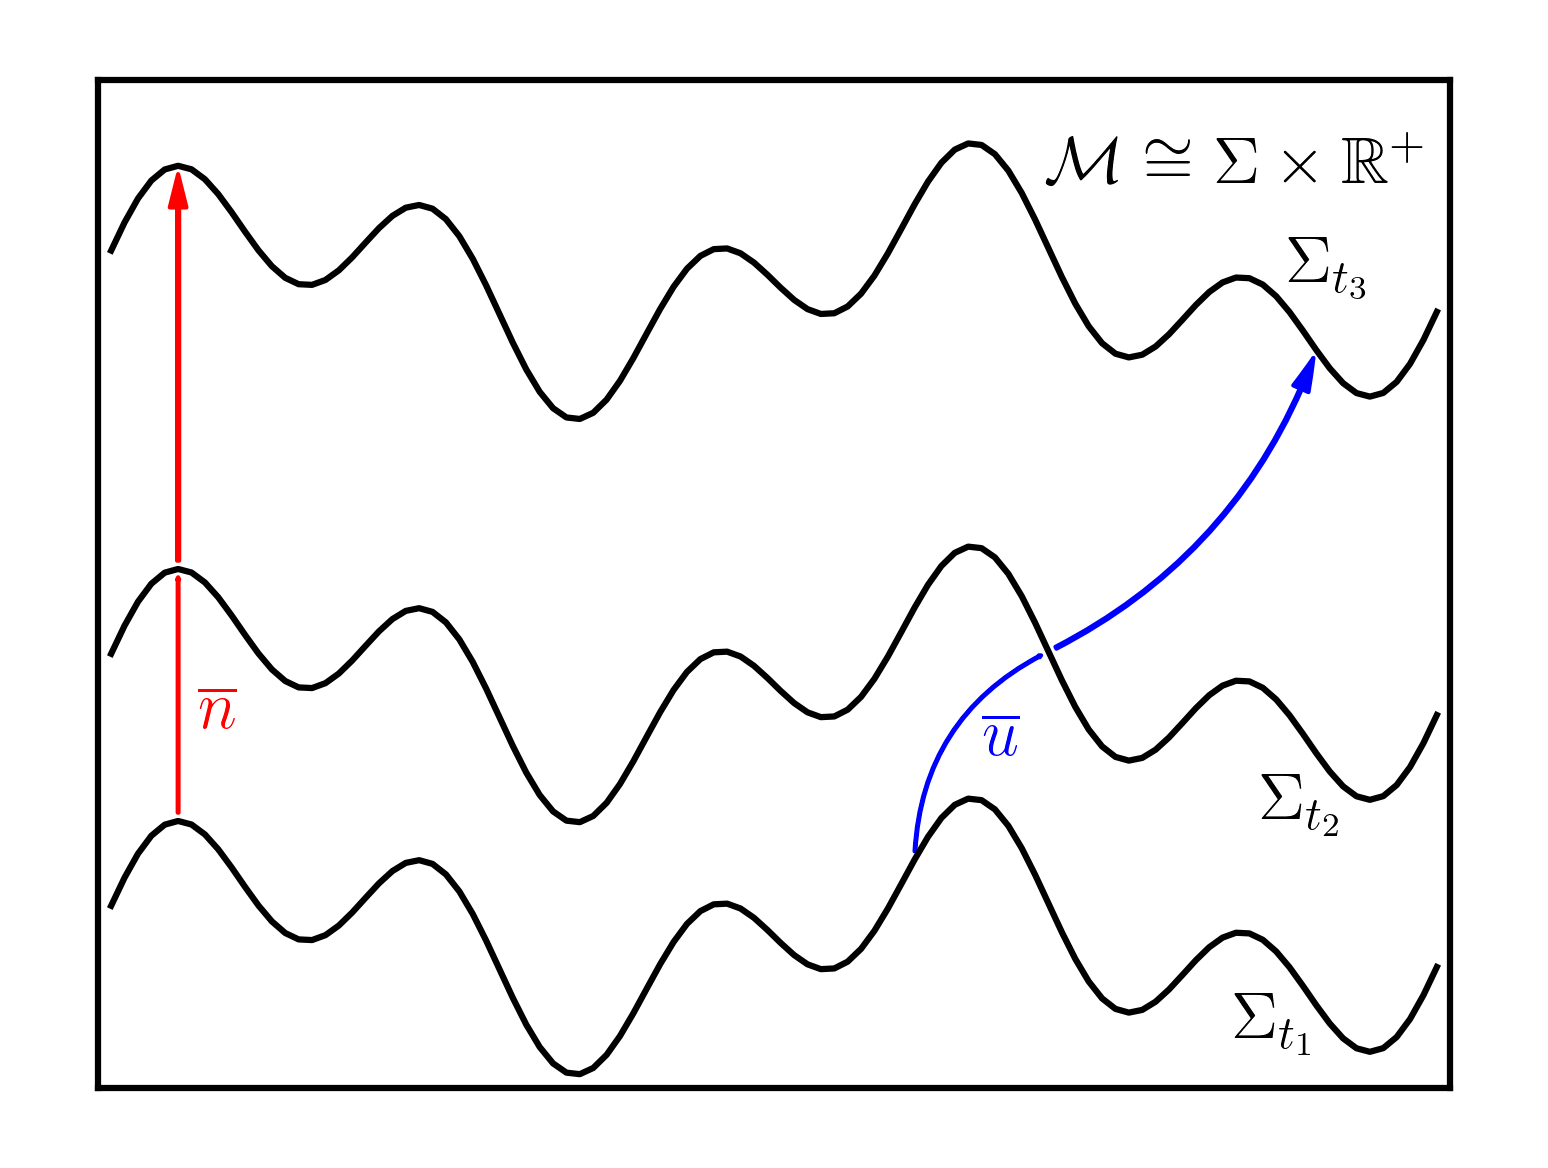
\includegraphics[width=0.8\textwidth]{1+1b.png}
  \end{figure}

\end{frame}

\begin{frame}
\frametitle{Fluid Equations}

  \begin{itemize}[<+->]
    \item[]
      Units defined such that $c=G=1$\\[1em]
    \item[]
      $\ol{\nabla}\cdot\ol{J}=0$\hspace{1em}
      ($\ol{J}$: baryon mass density current four-vector)
    \item[]
      $\ol{\nabla}\cdot\ol{\ol{T}}=\ol{0}$\hspace{1em}
      ($\ol{\ol{T}}$: Rank $\left(2,0\right)$ stress-energy tensor)\\[1em]
    \item[]
      $\ol{J}:=\rho\,\ol{u}$\hspace{1em}
      ($\rho$: \red{comoving} baryon mass density)\\[1em]
    \item[]
      $\ol{\ol{T}}:=\rho\,h\,\ol{u}\otimes\ol{u}+p\,\ol{\ol{g}}$\hspace{1em}
      ($p$: comoving thermal pressure,\\[0.5em]
      $h:=1+\left(e+p\right)/\rho$: specific enthalpy,
      $e$: comoving internal energy density)\\[1em]
    \item[]
      Five equations with six unknowns \frownie{}\\[1em]
    \item[]
      Close with an equation of state:
      $p=p\left(e\right):=\left(\Gamma-1\right)e$,
      $\Gamma=4/3$
  \end{itemize}

\end{frame}

\begin{frame}
\frametitle{Valencia Decomposition}

  \begin{figure}[htb!]
    \centering
    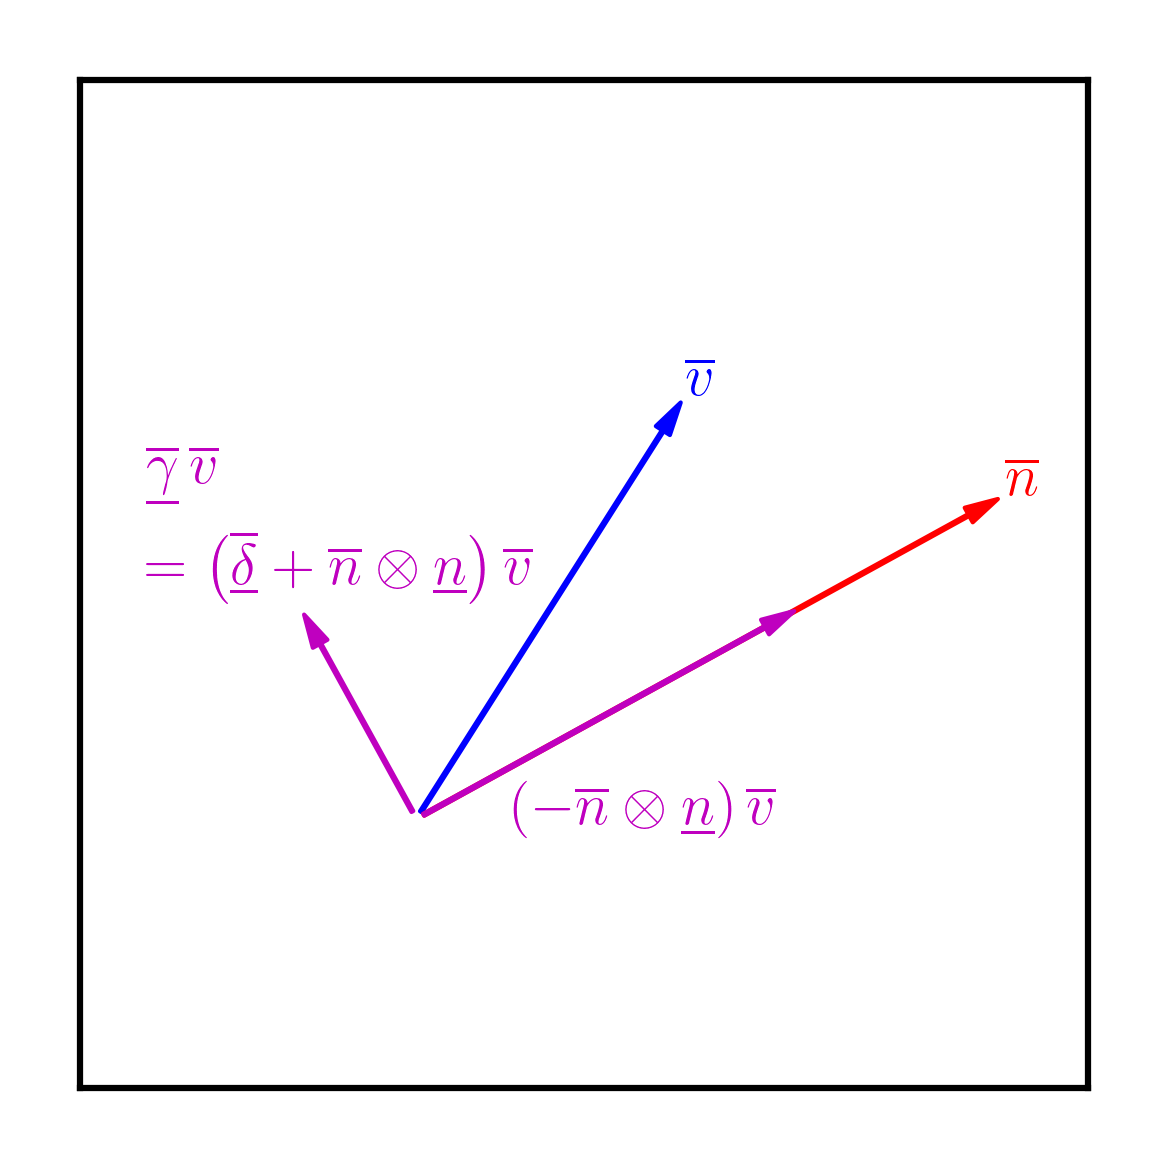
\includegraphics[width=0.6\textwidth]{decomp.png}
  \end{figure}

  \begin{itemize}[<+->]
    \item[]
     Extensible to higher-rank tensors!
  \end{itemize}

\end{frame}

\begin{frame}
\frametitle{Valencia Decomposition}

  \begin{itemize}[<+->]
    \item[]
      $E:=n_{\mu'}\,n_{\nu'}\,T^{\mu'\nu'}$\vspace{1em}
    \item[]
      $S^{\mu}:=-\gamma^{\mu}_{~\mu'}\,n_{\nu'}\,T^{\mu'\nu'}$\vspace{1em}
    \item[]
      $P^{\mu\nu}:=\gamma^{\mu}_{~\mu'}\,\gamma^{\nu}_{~\nu'}\,
      T^{\mu'\nu'}$\vspace{1em}
    \item[]
      Math...
  \end{itemize}

\end{frame}

\begin{frame}
\frametitle{Valencia Decomposition}

  \begin{equation*}
    \p_{t}\,\bs{U}
    +\frac{1}{\sqrt{\gamma}}\,
    \p_{i}\left[\alpha\,\sqrt{\gamma}\,\bs{F}^{i}\left(\bs{U}\right)\right]
    =\bs{S}\left(\bs{U}\right)
  \end{equation*}

  \begin{columns}[c]

    \column{.49\textwidth} % Left column and width

      \begin{itemize}[<+->]
        \item[]
          GR
        \item[]
          $\bs{U}:=\left(D,S_{j},\tau\right)^{\top}$
        \item[]
          $D:=\rho\,W$
        \item[]
          $S_{j}:=\rho\,h\,W^{2}\,v_{j}$
        \item[]
          $\tau:=E-D=\rho\,h\,W^{2}-p-\rho\,W$
        \item[]
          $\alpha=\left(1-\rsc/r\right)/\left(1+\rsc/r\right)$
        \item[]
          $\sqrt{\gamma}=\psi^{6}\,\sqrt{\bar{\gamma}}$
      \end{itemize}

    \column{.49\textwidth} % Left column and width

      \begin{itemize}[<+->]
        \item[]
          NR
        \item[]
          $\bs{U}:=\left(D,S_{j},\tau\right)^{\top}$
        \item[]
          $D:=\rho$
        \item[]
          $S_{j}:=\rho\,v_{j}$
        \item[]
          $\tau=e+\frac{1}{2}\,\rho\,v^{i}\,v_{i}$
        \item[]
          $\alpha=1$
        \item[]
          $\sqrt{\gamma}=\sqrt{\bar{\gamma}}$
      \end{itemize}

  \end{columns}

\end{frame}

\begin{frame}
\frametitle{Valencia Decomposition}

  \begin{equation*}
    \p_{t}\,\bs{U}
    +\frac{1}{\sqrt{\gamma}}\,
    \p_{i}\left[\alpha\,\sqrt{\gamma}\,\bs{F}^{i}\left(\bs{U}\right)\right]
    =\bs{S}\left(\bs{U}\right)
  \end{equation*}

  \begin{columns}[c]

    \column{.49\textwidth} % Left column and width

      \begin{itemize}
        \item[]
          GR
        \item[]
          $\bs{F}^{i}\left(\bs{U}\right)
          =\begin{pmatrix}
             \rho\,W\,v^{i} \\[1em]
             \rho\,h\,W^{2}\,v^{i}\,v_{j} + p\,\delta^{i}_{~j} \\[1em]
             \left(\rho\,h\,W^{2}-\rho\,W\right)\,v^{i}
           \end{pmatrix}$
      \end{itemize}

    \column{.49\textwidth} % Left column and width

      \begin{itemize}
        \item[]
          NR
        \item[]
          $\bs{F}^{i}\left(\bs{U}\right)
          =\begin{pmatrix}
             \rho\,v^{i} \\[1em]
             \rho\,v^{i}\,v_{j} + p\,\delta^{i}_{~j} \\[1em]
             \left(\rho\,h_{\nr}+\frac{1}{2}\,v^{j}\,v_{j}\right)\,v^{i}
           \end{pmatrix}$
      \end{itemize}

  \end{columns}

\end{frame}

\begin{frame}
\frametitle{Valencia Decomposition}

  \begin{equation*}
    \p_{t}\,\bs{U}
    +\frac{1}{\sqrt{\gamma}}\,
    \p_{i}\left[\alpha\,\sqrt{\gamma}\,\bs{F}^{i}\left(\bs{U}\right)\right]
    =\bs{S}\left(\bs{U}\right)
  \end{equation*}

\Fontvi

  \begin{columns}[c]

    \column{.49\textwidth} % Left column and width

      \begin{itemize}
        \item[]
          GR
        \item[]
          $\bs{S}\left(\bs{U}\right)=
          \begin{pmatrix}
          0 \\[1em]
          \frac{1}{2}\,\alpha\,P^{ik}\,\p_{j}\,\gamma_{ik}
            -E\,\p_{j}\,\alpha \\[1em]
          -S^{j}\,\p_{j}\,\alpha
          \end{pmatrix}$
      \end{itemize}

    \column{.49\textwidth} % Left column and width

      \begin{itemize}
        \item[]
          NR
        \item[]
          $\bs{S}\left(\bs{U}\right)=
          \begin{pmatrix}
          0 \\[1em]
          \frac{1}{2}\,P^{ik}\,\p_{j}\,\bar{\gamma}_{ik}
            -\rho\,\p_{j}\,\Phi \\[1em]
          -S^{j}\,\p_{j}\,\Phi
          \end{pmatrix}$
          $\Phi\left(r\right):=-M/r$
      \end{itemize}

  \end{columns}

\end{frame}

\section{Steady-State Solutions}

\begin{frame}
\frametitle{Steady-State Solutions (pre-shock)}

  \begin{equation*}
    \cancelto{0}{\p_{t}\,\bs{U}}
    +\frac{1}{\sqrt{\gamma}}\,
    \p_{r}\left[\alpha\,\sqrt{\gamma}\,\bs{F}^{r}\left(\bs{U}\right)\right]
    =\bs{S}\left(\bs{U}\right)
  \end{equation*}

  \begin{columns}[c]

  \column{.49\textwidth} % Left column and width

    \begin{itemize}[<+->]
      \item[]
        GR
      \item[]
        $\alpha\,\psi^{6}\,W\times4\pi\,r^{2}\,\rho\,v=-\mdot$
      \item[]
        $\alpha\,h\,W=\mathcal{B}$
      \item[]
        $p=K_{1}\,\rho^{\Gamma}$
    \end{itemize}

  \column{.49\textwidth} % Left column and width

    \begin{itemize}[<+->]
      \item[]
        NR
      \item[]
        $4\pi\,r^{2}\,\rho\,v=-\mdot$
      \item[]
        $\frac{1}{2}\,v^{2}+h_{\nr}+\Phi=\mathcal{B}_{\nr}$
      \item[]
        $p=K_{1}\,\rho^{\Gamma}$
    \end{itemize}

  \end{columns}

\end{frame}

\begin{frame}
\frametitle{Jump Conditions}

  \begin{columns}[c]

    \column{.4\textwidth} % Left column and width

      \begin{itemize}
        \item[]
          $\bs{U}_{1}\neq\bs{U}_{2}$
        \item[]
          $\bs{F}^{r}\left(\bs{U}_{1}\right)
          =\bs{F}^{r}\left(\bs{U}_{2}\right)$
        \item[]
          Yields:
        \item[]
          $\rho_{2}$
        \item[]
          $e_{2}\left(p_{2}\right)$
        \item[]
          $K_{2}\left(>K_{1}\right)$
        \item[]
          $v^{r}_{2}$
      \end{itemize}

    \column{.55\textwidth} % Left column and width

      \begin{figure}[htb!]
        \centering
        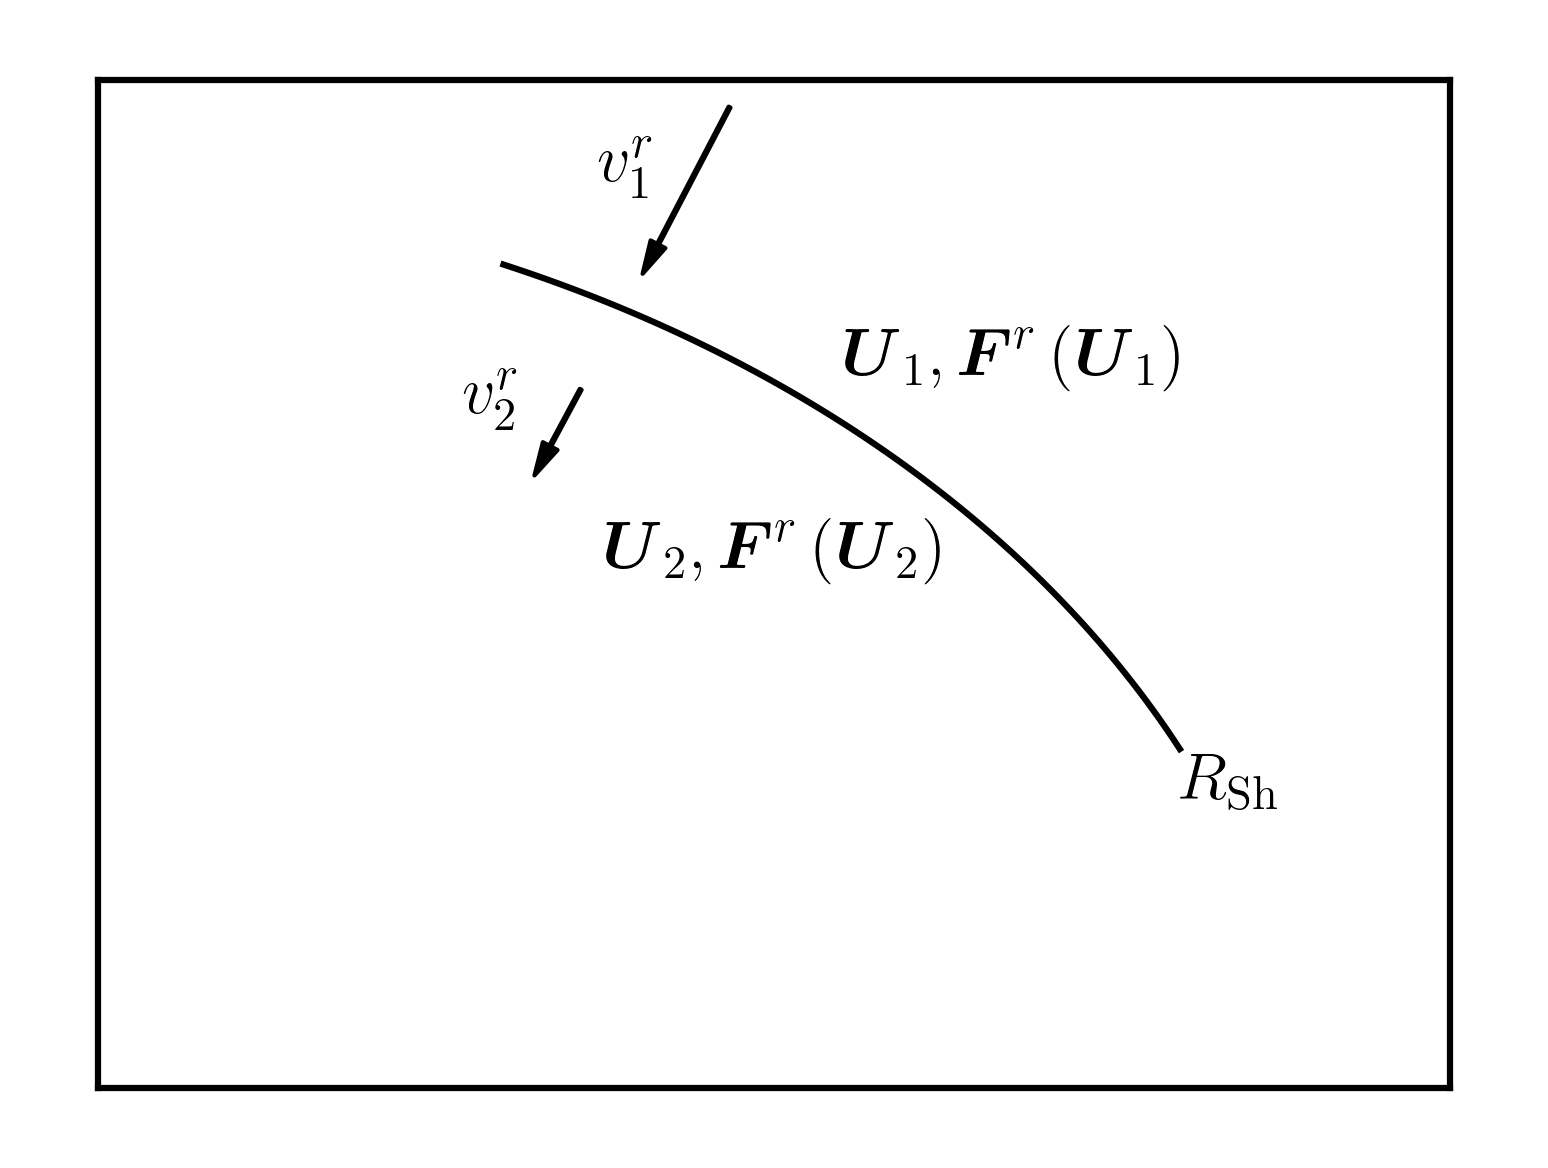
\includegraphics[width=\textwidth]{jump.png}
      \end{figure}

  \end{columns}

\end{frame}

\begin{frame}
\frametitle{Steady-State Solutions (post-shock)}

  \begin{equation*}
    \cancelto{0}{\p_{t}\,\bs{U}}
    +\frac{1}{\sqrt{\gamma}}\,
    \p_{r}\left[\alpha\,\sqrt{\gamma}\,\bs{F}^{r}\left(\bs{U}\right)\right]
    =\bs{S}\left(\bs{U}\right)
  \end{equation*}

  \begin{columns}[c]

    \column{.49\textwidth} % Left column and width

      \begin{itemize}
        \item[]
          GR
        \item[]
          $\alpha\,\psi^{6}\,W\times4\pi\,r^{2}\,\rho\,v=-\mdot$
        \item[]
          $\alpha\,h\,W=\mathcal{B}$
        \item[]
          $p=\red{K_{2}}\,\rho^{\Gamma}$
      \end{itemize}

    \column{.49\textwidth} % Left column and width

      \begin{itemize}
        \item[]
          NR
        \item[]
          $4\pi\,r^{2}\,\rho\,v=-\mdot$
        \item[]
          $\frac{1}{2}\,v^{2}+h_{\nr}+\Phi=\mathcal{B}_{\nr}$
        \item[]
          $p=\red{K_{2}}\,\rho^{\Gamma}$
      \end{itemize}

  \end{columns}

\end{frame}


\begin{frame}

  \begin{columns}[c]

    \column{.49\textwidth} % Left column and width

      \begin{itemize}
        \item[]
          $\eta\left(r\right):=\frac{r-\rpns}{\rsh-\rpns}$ \\[1em]
        \item[]
          $\frac{\delta p\left(\eta,\theta\right)}
                {p\left(\eta_{\mathrm{c}}\right)}
          =10^{-6}\times
           \exp\left[\frac{-\left(\eta-\eta_{\mathrm{c}}\right)^{2}}
                          {2\,\sigma^{2}}\right]
           \cos\theta$ \\ [1em]
          $\eta_{\mathrm{c}}=0.75$ \\ [1em]
          $\sigma=0.05$
      \end{itemize}

    \column{.5\textwidth} % Right column and width

      \begin{figure}[htb!]
        \centering
        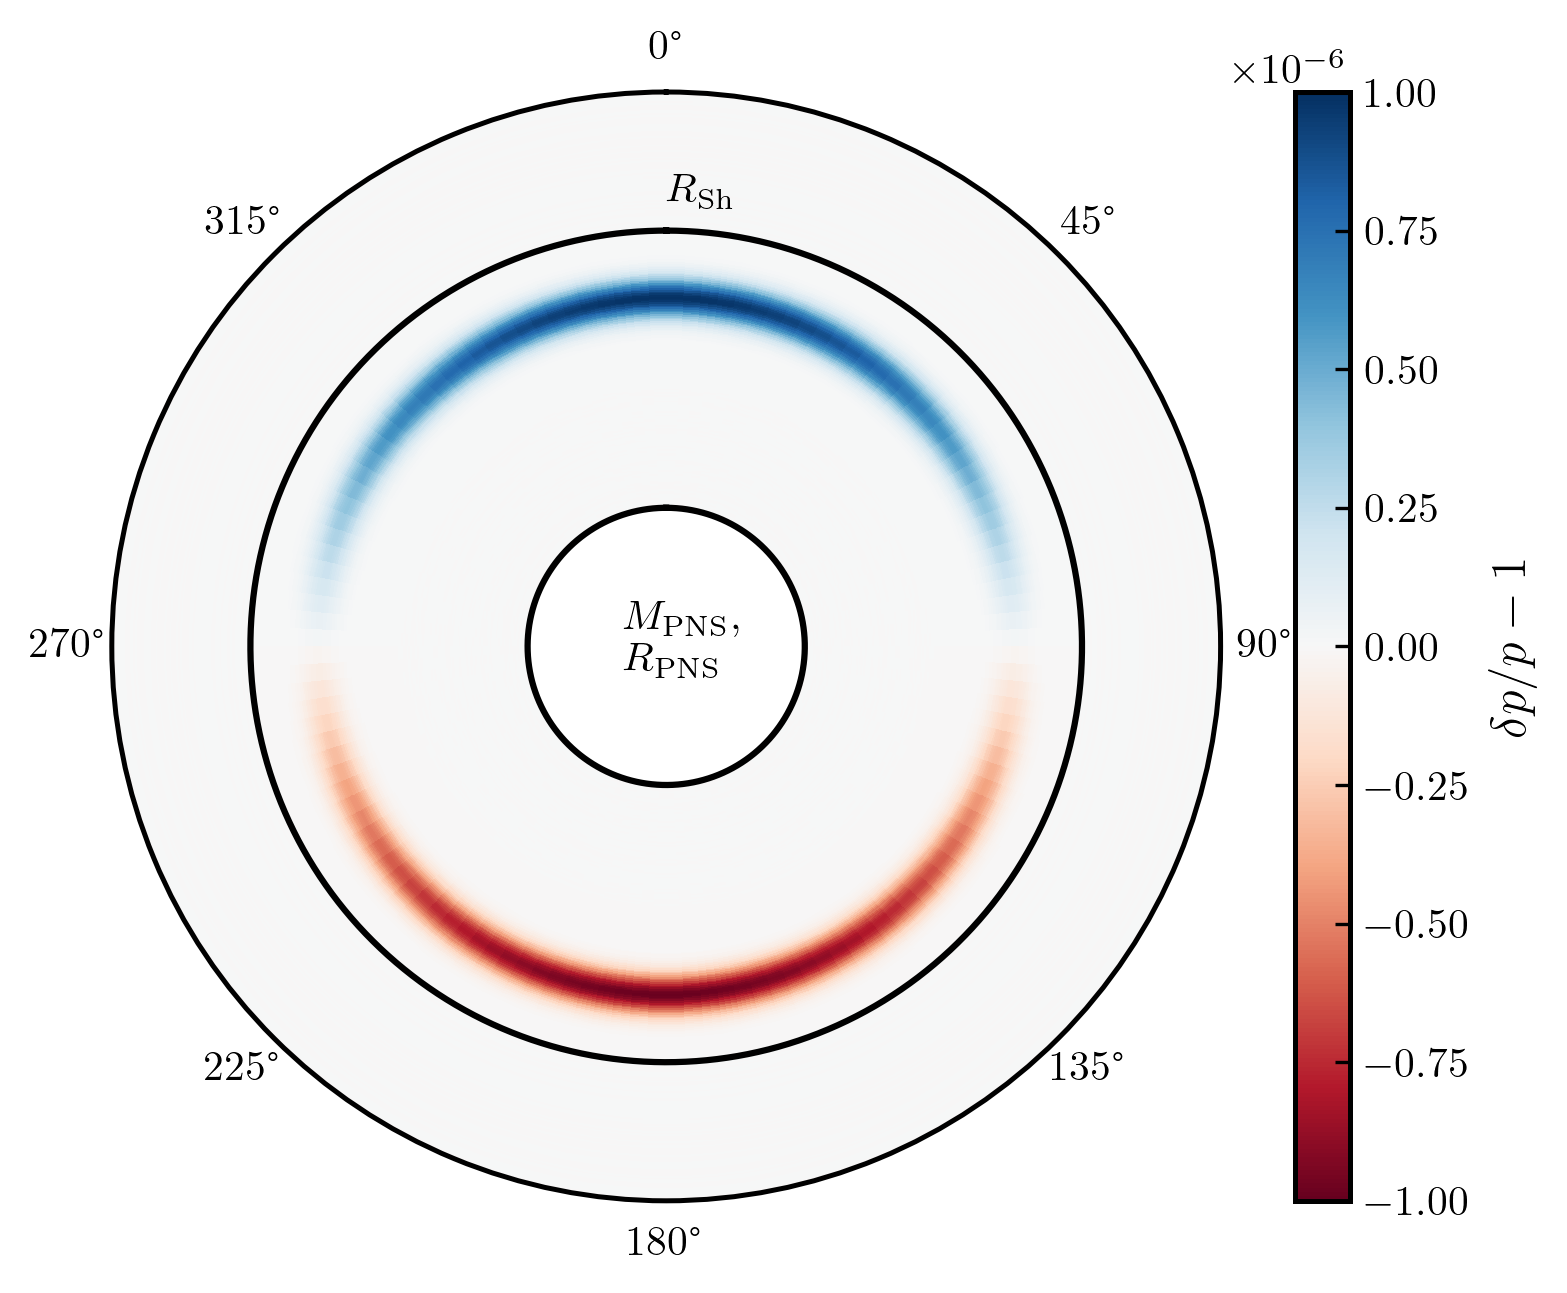
\includegraphics[width=\textwidth]{pert.png}
      \end{figure}

  \end{columns}

\end{frame}

\begin{frame}

  \begin{equation*}
    F\left(t\right)
      =F\left(0\right)\,
      e^{2\,\red{\omega}\,t}\,
      \sin^{2}\left(\frac{2\pi\,t}{\color{purple}{T}}+\delta\right)
  \end{equation*}
  \citep{bm2006}

  \begin{figure}[htb!]
    \centering
    \includegraphics[width=0.5\textwidth]%
    {fig.LegendrePowerSpectrum_vst_M1.4_Rpns040_Rsh1.20e2.png}
  \end{figure}

\end{frame}

\begin{frame}

  $F^{r}_{\theta}
  :=\alpha\,\psi^{6}\,h\,W^{2}\times
  \sqrt{\bar{\gamma}}\,\rho\,v^{r}\,v_{\theta}$ \\[1em]
  $\widetilde{F}^{r}_{\theta}:=\mathrm{FFT}\left\{F^{r}_{\theta}\right\}$

  \begin{figure}[htb!]
    \centering
    \begin{minipage}{0.45\textwidth}
      \includegraphics[width=\textwidth]%
      {fig.latFlux.png}
    \end{minipage}
    \hfill
    \begin{minipage}{0.45\textwidth}
      \includegraphics[width=\textwidth]%
      {fig.FFT_M2.8_Rpns020_Rsh6.00e1.pdf}
    \end{minipage}
  \end{figure}

  \begin{flushright}
  $T$ defined as the unique $\widetilde{T}$ such that
  $\widetilde{F}^{r}_{\theta}\left(\widetilde{T}\right)=1$
  \end{flushright}

\end{frame}

\begin{frame}

  \begin{figure}[htb!]
    \centering
    \begin{minipage}{\textwidth}
      \begin{minipage}{0.35\textwidth}
        \includegraphics[width=\textwidth]%
        {fig.LegendrePowerSpectrum_vst_M1.4_Rpns040_Rsh1.20e2.pdf}
      \end{minipage}
      \hfill
      \begin{minipage}{0.35\textwidth}
        \includegraphics[width=\textwidth]%
        {fig.LegendrePowerSpectrum_vst_M1.4_Rpns040_Rsh1.50e2.pdf}
      \end{minipage}
      \begin{minipage}{0.4\textwidth}
        \includegraphics[width=\textwidth]%
        {fig.FFT_M1.4_Rpns040_Rsh1.20e2.pdf}
      \end{minipage}
      \hfill
      \begin{minipage}{0.4\textwidth}
        \includegraphics[width=\textwidth]%
        {fig.FFT_M1.4_Rpns040_Rsh1.50e2.pdf}
      \end{minipage}
    \end{minipage}
  \end{figure}

\end{frame}

\end{document}
%------------------------------------------------------------------------------%
